%-------------------------------------------------------------------------------
% File: main.tex
%       Epidemic Broadcast project documentation.
%
%       Compile using:
%           $ pdflatex main.tex
%           $ biber main
%
% Author: Marco Pinna, Rambod Rahmani, Yuri Mazzuoli
%         Created on 05/12/2020
%-------------------------------------------------------------------------------
\documentclass[11pt, a4paper, twoside, openright]{book}

% equal left and right margins
\usepackage[hmarginratio=1:1]{geometry}

% configuration to typeset documents in italian
\usepackage[english]{babel}
\usepackage{import}
% include graphics in the file
\usepackage{graphicx}
\usepackage{pgf}
\usepackage{tikz}
% used in the dedication environment definition
\usepackage{afterpage}

% used to set page background image
\usepackage{tikz}

% used to handle math equations and formulas
\usepackage{amsmath}
\usepackage{mathtools}
\usepackage{array}

% used to handle quotes
\usepackage{csquotes}

%used to handle bibliography
\usepackage{biblatex}
\addbibresource{references.bib}

%used to change color and background color of single words
\usepackage{xcolor}

%used to place figures side by side
\usepackage{subfig}

%used to fix figure positioning
\usepackage{float}

%used to reference sections
\usepackage{hyperref}

\usepackage{wrapfig}

% blank page command
\newcommand{\blankpage}
{
    \null
    \thispagestyle{empty}%
    \addtocounter{page}{-1}%
    \newpage
}
\newcommand\inputpgf[2]{{
\let\pgfimageWithoutPath\pgfimage
\renewcommand{\pgfimage}[2][]{\pgfimageWithoutPath[##1]{#1/##2}}
\input{#1/#2}
}}
% dedication environment
\newenvironment{dedication}
{
    % blank page before dedication
    \afterpage{\blankpage}
    % we want a new page
    \clearpage
    % no header and footer
    \thispagestyle{empty}
    % some space at the top
    \vspace*{\stretch{1}}
    % the text is in italics
    \itshape
    % flush to the right margin
    \raggedleft
    % blank page after dedication
    \afterpage{\blankpage}
}
{
    % end the paragraph
    \par
    % space at bottom is one times that at the top
    \vspace{\stretch{1}}
    % finish off the page
    \clearpage
}

\newenvironment{specifications}
{
	\fontfamily{qtm}\selectfont
}{\par}

%-------------------------------------------------------------------------------
% Title page
%-------------------------------------------------------------------------------
\title{
    \vspace{-3cm}
    
\includegraphics[scale=0.3]{img/cherubino_black.eps}\\
    {\scshape University of Pisa}\\
    School of Engineering\\
    \rule{7cm}{0.01cm}\\
    {\normalsize{\scshape Performance Evaluation of Computer Systems and Networks}}\\
    [2cm]
    {\scshape Epidemic Broadcast}\\
    [3cm]
    \LARGE{\textbf{Supervisors}\hfill\textbf{Students}}\\
    \Large{\emph{Prof. Giovanni Stea}\hfill\emph{Marco Pinna\\}}
    \Large{\emph{Ing. Antonio Virdis}\hfill\emph{Rambod Rahmani\\}}
    \Large{\hfill\emph{Yuri Mazzuoli\\}}
    \vfill
    \date{\today}
}

% leave the author field ampty in the title page
\author{}

%-------------------------------------------------------------------------------
% Document beginning
%-------------------------------------------------------------------------------
\begin{document}

% make title page
\maketitle

% blank page before dedication
\afterpage{\blankpage}	

% enable page numbering back: roman numbers style
\pagenumbering{roman}

% print table of contents
\tableofcontents

% set arabic page numbering style
\pagenumbering{arabic}

%-------------------------------------------------------------------------------
% File: introduction.tex
%       Epidemic Broadcast project documentation.
%
% Author: Marco Pinna, Rambod Rahmani, Yuri Mazzuoli
%         Created on 05/12/2020
%-------------------------------------------------------------------------------
\chapter{Introduction}
In what follows the study on the broadcast of an epidemic message is carried
out.\\
The specifications are detailed in the following:
\begin{displayquote}
    \begin{specifications}
    {\Large Epidemic broadcast}\\
    Consider a 2D floorplan with \textit{N} users randomly dropped in it. A
    random user within the floorplan produces a \textit{message}, which should
    ideally reach all the users as soon as possible. Communications are
    \textit{slotted}, meaning that on each slot a user may or may not relay the
    message, and a message occupies an entire slot. A \textit{broadcast radius
    R} is defined, so that every receiver who is within a radius \textit{R} from
    the transmitter will receive the message, and no other user will hear it. A
    user that receives more than one message in the same slot will not be able
    to decode any of them (\textit{collision}). Users relay the message they
    receive \textit{once}, according to the following policy
    (\textit{p-persistent relaying}): after the user successfully receives a
    message, it keeps extracting a value from a Bernoullian RV with success
    probability \textit{p} on every slot, until it achieves success. Then it
    relays the message and stops. A sender does not know (or cares about)
    whether or not its message has been received by its neighbors.\\
    \\
    Measure at least the broadcast time for a message in the entire floorplan,
    the percentage of covered users, the number of collisions.\\
    \\
    In all cases, it is up to the team to calibrate the scenarios so that
    meaningful results are obtained.
    \end{specifications}
\end{displayquote}
The work is organized as follows:
\begin{itemize}
    \item Firstly, an initial overview and a presentation of the problem are
    given. Here, meaningful parameters to be tweaked and useful scenarios are
    identified and some considerations about them are made.
    \item Secondly, a graph-based modelling technique, commonly used in
    literature, is proposed and some simplified scenarios are analysed.
    \item Then, in Chapter \ref{modelling} the complete model is considered and
    some assumptions about it are made, such as its performance when one or more
    parameters are set to extreme values or its asymptotic behaviour with
    different configurations of the parameters.
    \item In chapter [TODO] the construction of the simulator is described and
    the results of its validation are presented.
    \item Chapter [TODO] concerns the full simulation and performance evaluation
    of the system.
\end{itemize}

%-------------------------------------------------------------------------------
% File: overview.tex
%       Epidemic Broadcast project documentation.
%
% Author: Marco Pinna, Rambod Rahmani, Yuri Mazzuoli
%         Created on 05/12/2020
%-------------------------------------------------------------------------------
\chapter{Overview}\label{ch:overview}
To perform the analysis of the broadcast of a message that should reach as many
users as possible in a 2D floorplan, the following hypotheses were made:
\begin{itemize}
	\item the floorplan always has a rectangular shape and it is empty, (i.e.
	there are no obstacles such as walls or pillars in it);
	\item each user is considered point-like and does not move inside the
	floorplan;
	\item the transmission of a message is instantaneous and it happens at the
	beginning of every time slot; the whole apparatus can therefore be
	considered a \textit{Discrete Time System}.
\end{itemize}
Depending on the performance metrics to be analysed, different choices can be
made about the parameters to be adjusted. According to the specifications, the
main three metrics for this study are:
\begin{itemize}
	\item the broadcast time \colorbox{gray!30}{\large \texttt{T}} for a message
	to cover as many user as possible in the entire floorplan; the effective
	duration of the transmissions slots obviously has an effect
	on the total broadcast time, but it is only a scaling factor on the total
	number of slots; \texttt{T} can therefore be measured in terms of slots and
	converted to units of time accordingly.
	\item the percentage of covered users \colorbox{gray!30}{\large \texttt{U}};
	\item the number of collisions \colorbox{gray!30}{\large \texttt{C}}:
	collisions are detected by nodes, they happen when a node receives more than
	one message in the same time slot; in order to measure the number of
	collisions;
\end{itemize}
The following parameters have been identified: the transmission range of the
users, the \textit{per-slot} transmission probability, the floorplan size and
its shape, and the density of users in the floorplan per square metre.\\
\\
To be more detailed:
\begin{itemize}
	\item the radius of transmission \colorbox{gray!30}{\large \texttt{R}}: it
	represents the maximum distance between two users such that the message
	sent from one is detected by the other; it is the same for every user on
	the floorplan.\\
	$R$ clearly has a great impact on all
    the performance metrics: the greater this radius, the faster the message
    moves across the floorplan and the higher the number of users that can be
    reached; on the other hand, a greater radius is likely to cause more
    collisions than a smaller one. \\
	 Realistic values for $R$ have been taken from Bluetooth Low
	Energy standard and range from a minimum of $5$ metres to a maximum of $20$
	metres.
	\item the \textit{per-slot} transmission probability
	\colorbox{gray!30}{\large \texttt{p}}: it is the success probability for the
	Bernoullian random variable associated to the transmission. As a
	probability, it can assume values between 0 and 1.\\
	The higher the transmission probability $p$, the faster a message ”moves away” from
a user; at the same time, a high transmission probability implies a high collision
probability in a local area where two or more nodes are transmitting;
    \item the length of the side of the floorplan rectangle
    \colorbox{gray!30}{\large \texttt{L}}; \\
    A bigger floorplan area, all else being equal, will require a longer
    time to be covered entirely by the broadcast;
	\item the \textit{aspect ratio} of the floorplan rectangle
	\colorbox{gray!30}{\large \texttt{a}}, defined as the ratio between the
	longer side $L$ and the shorter side $W$; because of the radial symmetry of
	the transmission phenomenon, there is no actual need to consider values for
	\texttt{a} lower than 1.\\
	A very long and very narrow floorplan will probably cause less collisions than a
square one with the same area, as the average number of users in the collision
range of a random user decreases; on the other hand, the performance of this type of
scenario will be highly influenced by the position of the starting node;

%TODO remove? Reprhase? We are already specifying that we only tweaked p and R
%	this parameter is fixed at 1 in our simulation model, 
%	so we are considering only square floorplans; this will allow the analysis
%	to be focused on more important parameters, but still in a quite common
%	scenario;
%TODO number of users is defined as number of users? Redundant? Remove definition? Rephrase?
	\item number of users \colorbox{gray!30}{\large \texttt{N}}, defined
	as the number of users dropped on the floorplan;
	\item users population density \colorbox{gray!30}{\large \texttt{d}},
	defined as the number of users per square meter; for this parameters, we
	decided to study two opposite density scenarios
	(high: 1/$m^2$ and low 0.1/$m^2$).
\end{itemize}

For this study, the two main parameters were \colorbox{gray!30}{\large \texttt{R}} and \colorbox{gray!30}{\large \texttt{p}}. Full sweeps for different values of both were made. \\
\colorbox{gray!30}{\large \texttt{a}} was kept constant and equal to 1 (i.e. the floorplan is always a square) and \colorbox{gray!30}{\large \texttt{L}} was either $10 m$ (``small" configuration) or $100 m$ (``big" configuration). \colorbox{gray!30}{\large \texttt{N}} was also kept constant and equal to 100.

%-------------------------------------------------------------------------------
% File: modelling.tex
%       Epidemic Broadcast project documentation.
%
% Author: Marco Pinna, Rambod Rahmani, Yuri Mazzuoli
%         Created on 05/12/2020
%-------------------------------------------------------------------------------
\chapter{System modelling}\label{modelling}
Wireless communication networks have been extensively studied in scientific
literature and one of the most used mathematical tools to model them and their
behaviour is \textit{graph theory}. In this work the same approach was used.\\
If we think of the users involved in the broadcasting of the message as the
nodes of a graph, as the broadcast propagation goes on and the message is
transmitted among the nodes, the system goes through different states where each
node could be either transmitting, listening or stopped.
We can therefore think of the state of the entire system as a combination of
the states of each node. The different nodes behaviours were modelled by means
of three different states:
\begin{itemize}
	\item \texttt{listening}: the node has not received the broadcast message
	yet and therefore it is still listening for incoming messages from other nodes;
	\item \texttt{transmitting}: the node has received the message and during
	each time slot it is trying to transmit it to adjacent nodes; in what
	follows, a node in \texttt{transmitting} state will be referred to as
	\textit{active} node;
	\item \texttt{sleeping}: the node has already received the message and
	retransmitted it; once a node is in a \texttt{sleeping} state, it will
	remain in such state and will therefore have no	effect on the system any more.
\end{itemize}
\section{Graph model for wireless systems}
The $N$ users dropped on the floorplan make up the set of vertices $V$ of a
graph $G$, whose set of edges $E$ is composed by all the connections between
each two nodes in reach of one another. Consider the following as a simplified
scenario to exemplify this model.
\begin{figure}[H]
	\begin{minipage}{.5\textwidth}
        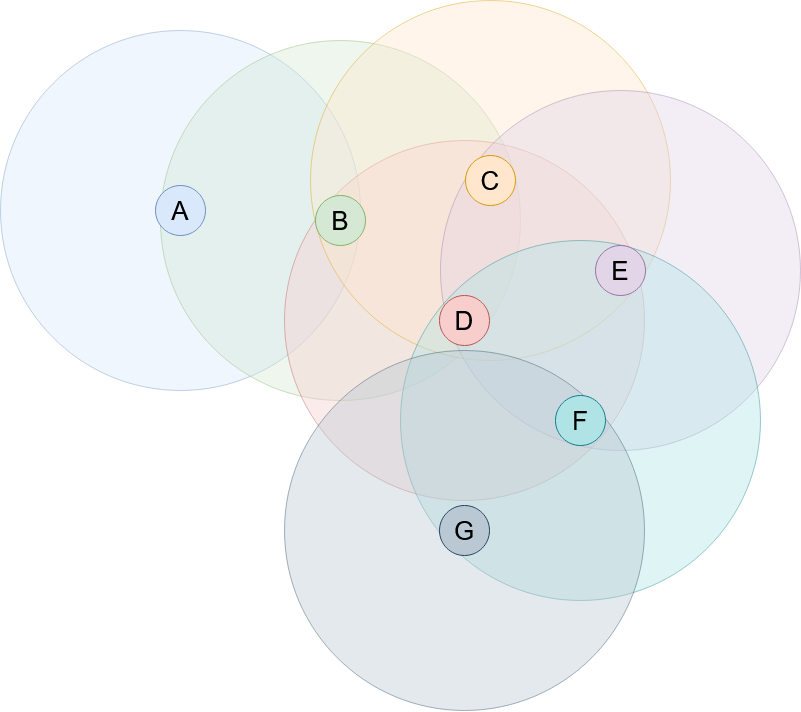
\includegraphics[scale=.23]{img/wireless_graph_1.png}
        \begin{center}
            a) Ranges representation
        \end{center}
	\end{minipage}
	\begin{minipage}{.5\textwidth} 
		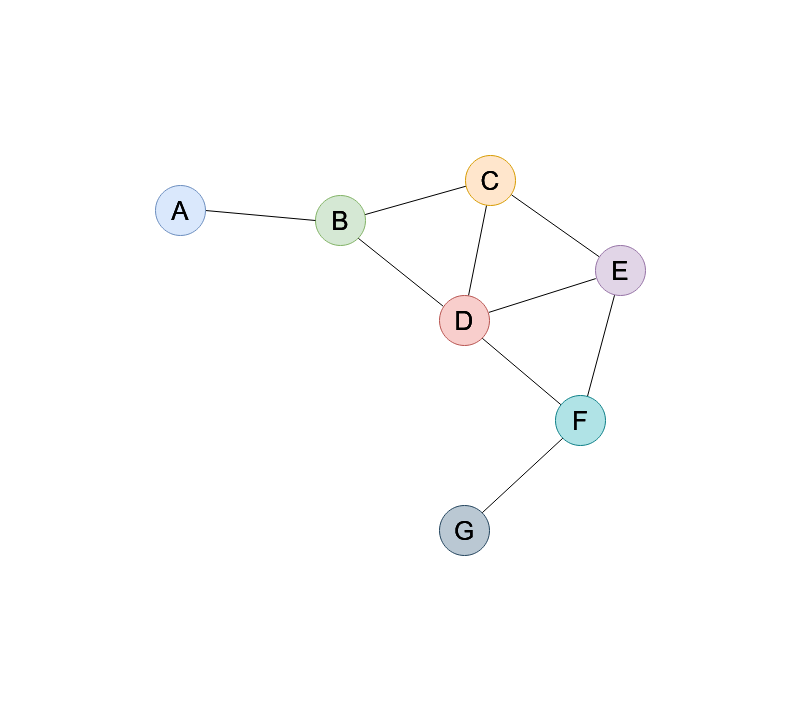
\includegraphics[scale=.23]{img/wireless_graph_2.png}
		\begin{center}
            b) Equivalent graph representation
        \end{center}
	\end{minipage}
	\caption{}
    \label{fig:graph1}
\end{figure}
\noindent In figure \ref{fig:graph1} (a) devices A, C and D are within device B
transmission radius. In the equivalent graph, there will be edges that connect
B to A, to C and to D. The same goes for all the other vertices. The resulting
graph is shown in figure \ref{fig:graph1} (b).\\
In general, the existence of an edge from vertex $i$ to vertex $j$ means that
nodes $i$ and $j$ are within reach of each other. Two vertices connected by an
edge are said to be \textit{adjacent}. The set composed by the vertex $v$
together with all its adjacent vertices form a subgraph called the
\textit{neighbourhood of v}.\\
During the broadcast, a node can only receive from and transmit to its
neighbourhood.\\
\\
Once a node has transmitted the message and has gone into \texttt{sleeping}
state, it disappears, along with all the edges connected to it. Therefore, the set of vertices V changes with time. This is what in literature is called a \textit{dynamic graph} or, more specifically, a \textit{node-dynamic graph.}

%Should this paragraph be moved to another chapter/section ?
Modelling the system with graphs also allows for the easy computation of a lower bound for the broadcast time \texttt{T}, which can be useful for the validation of the simulator.\\
Given a graph $G(V, E)$ that represents the users in the floorplan, let $v^{*}$ be the starter of the broadcast, i.e. the first node with the message.\\
In a best case scenario, the system evolves with no collisions at all and the message moves along the paths of the graph, reaching all nodes.\\
%TODO add citation to bibliography: [ F. Harary, Graph Theory, Addison-Wesley, 1969, p.199. ]
Let $d(u, v)$ be the \textit{distance} between two vertices $u$ and $v$, i.e. the length of a shortest directed path from u to v consisting of arcs, provided at least one such path exists.\\
Then, the lower bound for the broadcast time is given by the greatest distance between $v^{*}$ and any other vertex. This quantity, in graph theory, is called \textit{eccentricity} of the vertex $v^{*}$. More formally, the eccentricity of $v^{*}$ is defined as follows:

\begin{equation}
\epsilon(v^{*}) = \max_{v{\in}V} d(v^{*}, v)
\end{equation}



\section{Simplified models}

\subsection{Single queue configuration}\label{ssec:singlequeue}

Let us consider a configuration where devices arranged in a line, as shown in Fig. \ref{fig:single_queue}. Each device only has two neighbours, except for the outer ones that only have one. Let assume A to be the broadcast starter. A is in \texttt{transmitting} state while all the other nodes are initially in \texttt{listening} state. 
\hfill \break
\hfill \break

\begin{figure}[H]%
    \centering
	{{
\includegraphics[scale=0.6]{img/single_queue.png} }}%
    \caption{}%
    \label{fig:single_queue}%
\end{figure}

It is clear that, with this configuration, each listening node has a maximum of one active node in its neighbourhood and thus cannot possibly receive the message from two different sources at the same time.
This guarantees the absence of collisions.

In such a scenario, $100\%$ asymptotic coverage is ensured:
during each slot, the active node extracts a Bernoulli RV with success probability $p$. The probability of the active node not transmitting for k consecutive slots is a geometric distribution:

\begin{equation}
	P(X = k) = (1\text{-}p)^{k}
	\label{geometric_distribution}
\end{equation}

The successful transmission of the message from an active node to its neighbour is thus guaranteed since $\lim_{k \to \infty} (1\text{-}p)^{k} = 0$

%TODO not really sure about this result when the starter node is not the first or the last. What if the starter node is in the middle of the queue?
As for the total broadcast time \texttt{T}, on average it is equal to the mean value of the Bernoulli RV, \textit{p}, times the number of hops needed to reach the last node.
%times the eccentricity of the starter, maybe? Not really sure about that, I have to look into it a bit more in detail

\begin{equation}
	E[T] = p \cdot (N-1)
	\label{singleQueueMeanT}
\end{equation}

\subsection{Star configuration with one active node}
Another useful simple configuration worth analysing is a star-shaped configuration. In this setup, there is a central node A connected to N-1 nodes, all of which are non-adjacent to each other. Let us suppose A to be the broadcast starter.

\begin{figure}[H]%
    \centering
	{{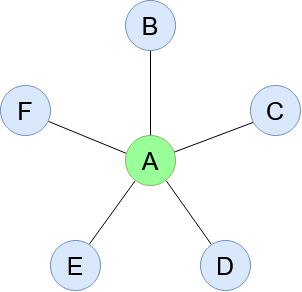
\includegraphics[scale=0.5]{img/star_graph.png} }}%
    \caption{}%
    \label{fig:star_graph}%
\end{figure}

The absence of collisions is ensured in this scenario as well, for the same reason as the previous example.\\
At each slot, A keeps extracting a Bernoulli RV. When the extraction is successful, A broadcasts the message to all its neighbour and total coverage is reached. Hence, 100\% asymptotic coverage is ensured in this case too, as the probability of A not transmitting for k consecutive slots is Eq. \ref{geometric_distribution} and goes to 0 as k goes to infinity.\\
In this case, the average total broadcast time E[\texttt{T}] is simply equal to the mean value of the Bernoulli RV \textit{p}.

If the broadcast starter was one of the ``rays" of the star, instead of the center, there would not be much difference: absence of collisions and total coverage would be ensured as well.\\
As for \texttt{T}, its expected value would just be $2p$, since the are now \textbf{two} hops involved in the broadcast: one from the starter to the center of the star and the other from the center node to all the N-2 remaining ones.

\subsection{Star configuration with all but one active nodes}
\label{ssec:star2}

This configuration can be seen as the complement of the previous one: every ``ray" of the star is active and trying to transmit the message to the center node.

\begin{figure}[H]%
    \centering
	{{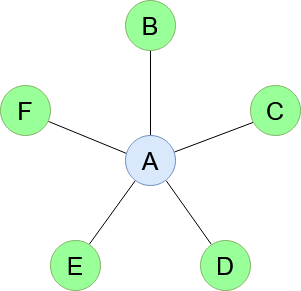
\includegraphics[scale=0.5]{img/star_graph2.png} }}%
    \caption{}%
    \label{fig:star_graph}%
\end{figure}

Now there is the possibility of collisions and a non-zero probability that there will never be total coverage.

To simplify the analysis of this system and obtain some more insight, it is useful to model it by means of a discrete-time Markov chain.

%TODO choose better title for subsection, maybe?
\subsubsection{Discrete-time Markov chain model for N nodes transmitting to a target}
Since the state of the system evolves only once per slot, it can be modelled with a discrete-time Markov chain (DTMC).
\hfill \break
\hfill \break

\begin{figure}[H]%
    \centering
	{{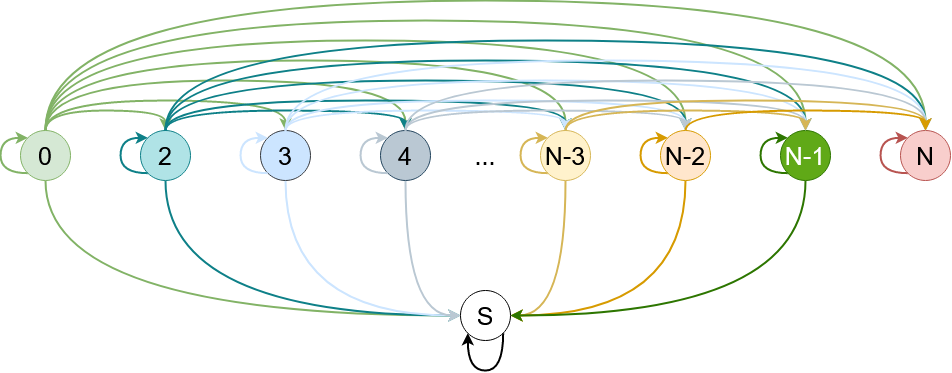
\includegraphics[scale=0.4]{img/DTMC.png} }}%
    \caption{Discrete-time Markov chain for a scenario with N active devices}%
    \label{fig:dtmc}%
\end{figure}

\noindent Figure \ref{fig:dtmc} shows the DTMC for a generic configuration with N transmitters (transition probabilities are not shown for the sake of clarity).\\
State 0 and states 2 to N represent the number of \texttt{sleeping} devices, namely devices that have already sent the message and have stopped. 
State S represents the successful transmission state, which the system transitions to when only one device has transmitted the message during the previous slot.

The initial state $X_{0}$ is 0. Any transition from a state $i$ to a state $j$, $j \neq S$, means that more than one device has transmitted the message and consequently the target device has detected a collision.
Both state S and state N are \textit{absorbing states}, i.e. states that, once entered, cannot be left (as can be seen in Fig. \ref{fig:dtmc}, where the only outgoing arrow from each of the two goes back to the state itself).

If the system transitions to state N, it stays in it indefinitely since all the devices would be \texttt{sleeping} and they cannot become active again. This implies that there will never be total coverage since the target device will forever stay in a \texttt{listening} state.\\
%TODO improve? Is it clear?
On the other hand, state S, although being an absorbing state as well, should actually be considered an ``exit" instead of a ``sink": if the system transitions to it, the target device has successfully received the message and the DTMC does not model the system any more.\\
Another interesting observation concerns state N-1: once the system reaches this state, it would be guaranteed that the target device will sooner or later receive the message, for the same reason set forth in \ref{ssec:singlequeue}.

\subsubsection{Transition probabilities}

Let us now address the challenging part: computing the transition probability.
\hfill \break
During the first slot, the probability that $j$ devices out of $N$ transmit the message is the following:

\begin{equation}
	P_{1}(j, N) = {N\choose j} p^{j} (1-p)^{N-j}
	\label{eq:firstSlotTransProb}
\end{equation}

\noindent Derivation of \ref{eq:firstSlotTransProb} can be found in Appendix A.\\

As for the probability of $j$ devices transmitting at the same time during slot $k$, be it $P_{k}(j)$, we can model the system as if it was in the first slot, with the total number of active devices now being equal to $N$ - $t$, where $t$ is the total number of devices that have transmitted up to the $(k\text{-}1)$-th slot.\\
%TODO fix
The problem with this formulation is... Is what? \\

A better way to compute the probability of having $j$ devices transmitting at slot $k$, is to use the \textit{stochastic matrix} of the Markov chain.

If the probability of moving from state $i$ to $j$ in one time slot is $Pr(j|i) = P_{i,j}$, the stochastic matrix P is given by using $P_{i,j}$ as the i-th row and j-th column element, e.g.

\begin{equation*}
P = 
\begin{bmatrix}
P_{0,0}	& P_{0,S}	& P_{0,2}	& \dots  	& P_{0,j}	& \dots		& P_{0,N} \\
P_{S,0}	& P_{S,S}	& P_{S,2}	& \dots  	& P_{S,j}	& \dots		& P_{S,N} \\
P_{2,0}	& P_{2,S}	& P_{2,2}	& \dots  	& P_{2,j}	& \dots		& P_{2,N} \\
\vdots	& \vdots	& \vdots	& \ddots 	& \vdots	& \ddots	& \vdots \\
P_{i,0}	& P_{i,S}	& P_{i,2}	& \dots		& P_{i,j}	& \dots		& P_{i,N} \\
\vdots	& \vdots	& \vdots	& \ddots	& \vdots	& \ddots	& \vdots \\
P_{N,0}	& P_{N,S}	& P_{N,2}	& \dots		& P_{N,j}	& \dots		& P_{N,N} \\
\end{bmatrix}
\label{stochasticMatrix1}
\end{equation*}
\hfill \break
Since S and N are absorbing states, $P_{S,j}=0$ for j $\neq$ S and $P_{N,j}=0$ for j $\neq$ N.\\
Moreover, all the possible transitions can only generate a non-decreasing sequence of states, hence $P_{i, j} = 0 $ $ \forall i > j $.\\
All the other elements of the matrix can be computed using formula \ref{eq:firstSlotTransProb}:

 \begin{equation}
	P_{i,j} = {N-i\choose j} p^{j} (1-p)^{N-i-j}
	\label{eq:matrixElementProb}
\end{equation}
\hfill \break
Therefore the stochastic matrix becomes:

\begin{equation*}
P = 
\begin{bmatrix}
P_{0,0}	& P_{0,S}	& P_{0,2}	& \dots  	& P_{0,j}	& \dots		& P_{0,N} \\
0		& 1			& 0			& \dots  	& 0			& \dots		& 0		 \\
0		& P_{2,S}	& P_{2,2}	& \dots  	& P_{2,j}	& \dots		& P_{2,N} \\
\vdots	& \vdots	& \vdots	& \ddots 	& \vdots	& \ddots	& \vdots \\
0		& P_{i,S}	& 0			& \dots		& P_{i,j}	& \dots		& P_{i,N} \\
\vdots	& \vdots	& \vdots	& \ddots	& \vdots	& \ddots	& \vdots \\
0		& 0			& 0			& \dots  	& 0			& \dots		& 1		 \\
\end{bmatrix}
\label{stochasticMatrix2}
\end{equation*}
\hfill \break
Let $x_{0}$ be the \textit{initial state vector}, i.e. an $N \times 1$ vector that describes the probability distribution of starting at each of the N possible states.\\
To compute the probability of transitioning to state $j$ in \textbf{k} steps, it is now sufficient to multiply the initial state vector $x_{0}$ by the stochastic matrix raised to the k-th power, e.g.

\begin{equation}\label{probAtStateK1}
P_{k}(j) = x_{0}\cdot P^{k}
\end{equation}
\hfill \break
In our case, the system always starts in state 0, so we have

\begin{equation*}
x_{0} = 
\begin{bmatrix}
1 \\
0 \\
0 \\
\vdots \\
0
\end{bmatrix}
\label{initialStateVector}
\end{equation*}
\hfill \break
which yields

\begin{equation}
P_{k}(j) = 
\begin{bmatrix}
1 \\
0 \\
0 \\
\vdots \\
0
\end{bmatrix}
\cdot P^{k} = (P^{k})_{0,j}
\label{eq:Pk_of_j}
\end{equation}
\hfill \break

Calculating the k-th power of a matrix can be an intensive task from a computational point of view. To improve the complexity of the computation, rows and columns of P can be rearranged, moving the S row and the S column as penultimate, thus obtaining

\begin{equation*}
P = 
\begin{bmatrix}
P_{0,0}	& P_{0,2}	& P_{0,3}  	& \dots	& P_{0, N-1}	& P_{0,S}	& P_{0,N} \\
		& P_{2,2}	& P_{2,3}  	& \dots	& P_{2, N-1}	& P_{2,S}	& P_{2,N} \\
		& 			& P_{3,3}	& \dots	& P_{3, N-1}	& P_{3,S}	& P_{3,N} \\
 		& 			& 			& \ddots& \vdots		& \vdots	& \vdots \\
		& 			& 			& 		& P_{N-1,N-1}	& P_{N-1,S}	& P_{N-1, N}\\
		& 			& 			& 		& 				& 1			& 0		 \\
0		& 			& 		  	& 		& 				& 			& 1		 \\
\end{bmatrix}
\label{triangularPMatrix}
\end{equation*}
\hfill \break

P is now an upper triangular matrix and this allows for faster computation of its powers in \ref{eq:Pk_of_j} .


%TODO add something about the number of collisions maybe?

%%-------------------------------------------------------------------------------
% File: complete_model_analysis.tex
%       Epidemic Broadcast project documentation.
%
% Author: Marco Pinna, Rambod Rahmani, Yuri Mazzuoli
%         Created on 05/12/2020
%-------------------------------------------------------------------------------
\chapter{Complete Model}\label{real_model_analysis}

%calcolare probabilità di un nodo di cadere nel range di un altro nodo

% calcolare la densità minima per cui mediamente c'è una distanza minore di R tra i nodi

%-------------------------------------------------------------------------------
% File: simulator.tex
%       Epidemic Broadcast project documentation.
%
% Author: Marco Pinna, Rambod Rahmani, Yuri Mazzuoli
%         Created on 05/12/2020
%-------------------------------------------------------------------------------
\chapter{Simulator}\label{simulator}
In order to obtain experimental results for the presented scenarios, a simulator
was built using OMNeT++ with the support of the INET framework. This allowed us
to reproduce the different scenarios, presented in the previous chapters, with
different values for the identified parameters.\\
\section{Omnet++ and INET framework}
OMNeT++ is an extensible, modular, component-based C++ simulation library and
framework, primarily for building network simulators\footnote{https://omnetpp.org/}.\\
The INET Framework is an open-source model library for the OMNeT++ simulation
environment. It provides protocols, agents and other predefined models for
researchers and students working with communication networks. INET is especially
useful when designing and validating new protocols, or exploring new or exotic
scenarios\footnote{https://omnetpp.org/download-items/INET.html}.\\
\\
OMNeT++ is a library and a framework, and can be used with the dedicated IDE.
Not only it allows for development of the simulator itself, but also to export
simulation results and to inspect simulation behaviour with a graphical user
interface. By taking advantage of the C++ compiler optimizations, it can achieve the lowest
%riformulare o spostare ?
% inoltre 'the lowest possible' forse è un po' azzardato da scrivere
% dato che non possiamo provare che non ci siano altri modi più veloci
simulation duration possible.

Networks are composed by modules; there are two
types of modules: simple module and compound module (which can contain other
modules itself).
INET, on the other hand, is an extension of OMNeT++, dedicated to recreating 
network simulation environments, with the capability of reproducing the activity
of a wireless communication system across multiple nodes. It contains ready to
use definitions and implementations of network related modules.\\
The INET framework was chosen in order to avoid spending too
much time on the coding side and therefore be able to focus more on other
aspects such as the problem modelling and analysis.
\section{Network architecture}
The network based architecture is composed by an array of \texttt{Host} modules, an
\texttt{Integrated visualizer} (visualizer) and a \texttt{UnitDiskRadioMedium} (radioMedium);
\begin{figure}[H]
    \begin{center}
        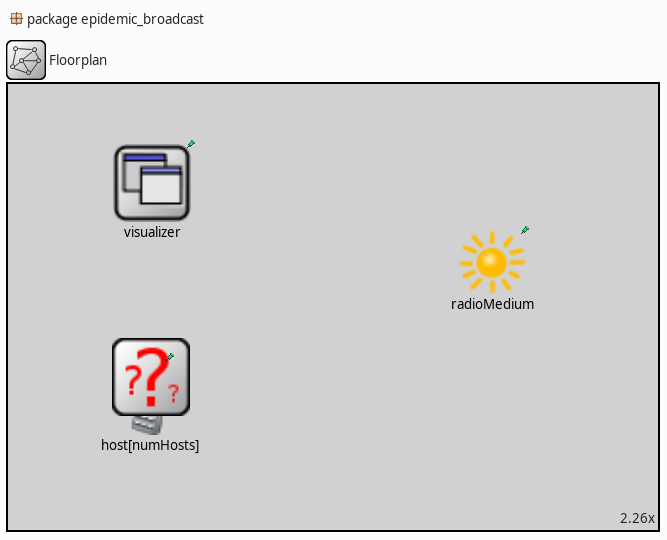
\includegraphics[scale=0.35]{img/floorplan.png}
        \caption{Floorplan.ned}
        \label{fig:floorplanOmnet}
    \end{center}
    \vspace*{-0.8cm}
\end{figure}
\begin{itemize}
    \item \textbf{UnitDiskRadioMedium} is a compound module provided by INET.
    This radio medium model provides a very simple but fast and predictable
    physical layer behaviour. It must be used in conjunction with the
    \texttt{UnitDiskRadio} model. It can simulate the behaviour of the wireless
    communication channel with various levels of abstraction.
    \item \textbf{Integrated visualizer} is a compound module provided by INET.
    It's resposible for the visual representation of modules properties and
    events in the graphic user interface.
    \item \textbf{Host} is the compound module developed to represent a node
    in the network environment.
\end{itemize}
The \texttt{Host} module extends the NodeBase module defined by INET. This
module contains the most basic infrastructure for network nodes that is not
strictly communication protocol related. The following diagram shows usage
relationships between types:
\begin{figure}[H]
    \begin{center}
        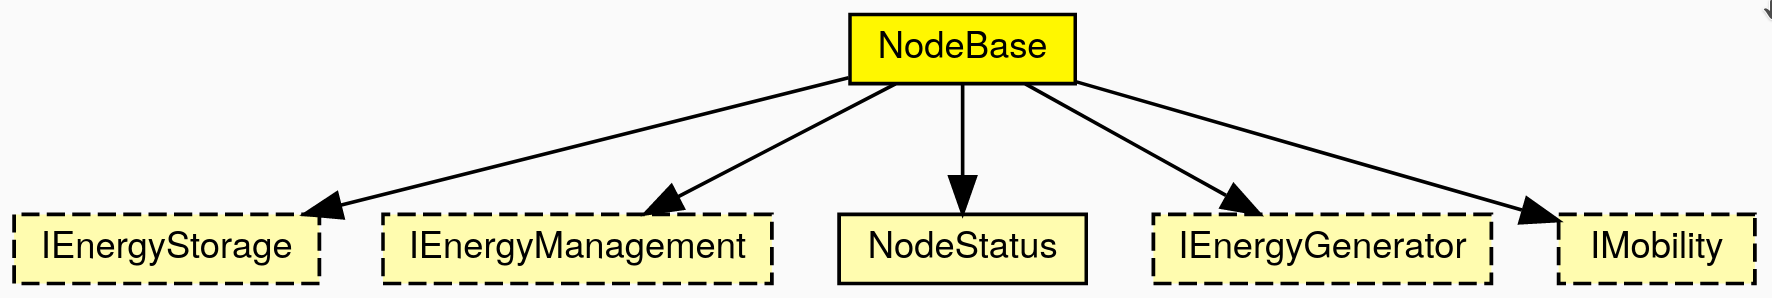
\includegraphics[scale=0.26]{img/nodebase.png}
        \caption{NodeBase Diagram.}
        \label{fig:nodebaseOmnet}
    \end{center}
    \vspace*{-0.8cm}
\end{figure}
\begin{figure}[H]
    \begin{center}
        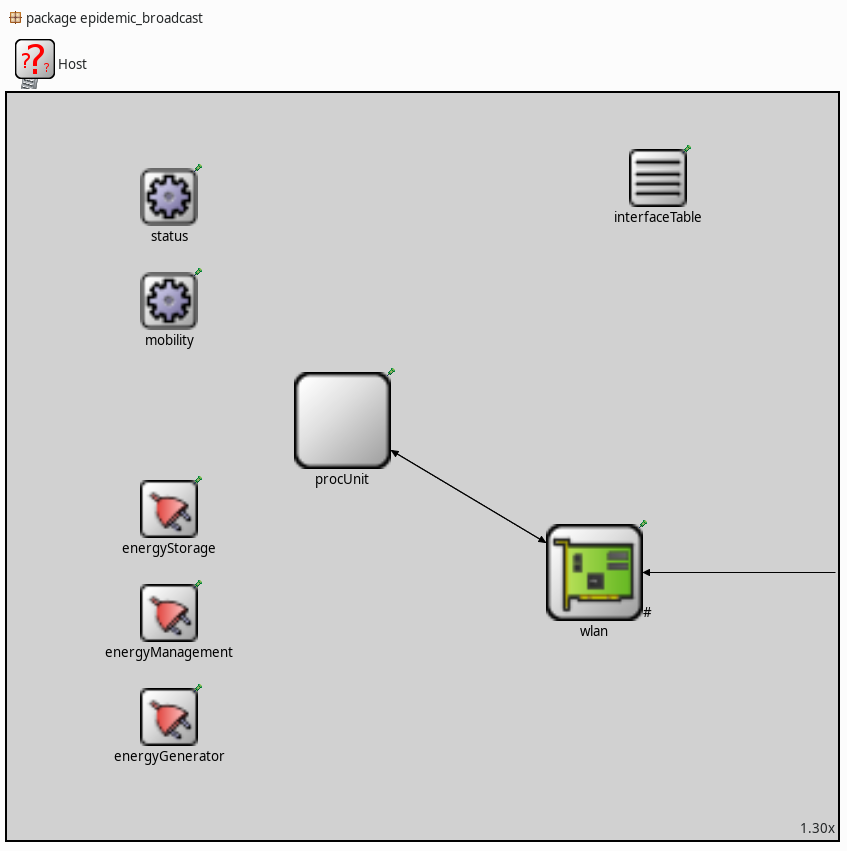
\includegraphics[scale=0.35]{img/host.png}
        \caption{host.ned}
        \label{fig:hostOmnet}
    \end{center}
    \vspace*{-0.8cm}
\end{figure}
\begin{itemize}
    \item the \texttt{mobility} module privided by INET manages the position of
    the parent module \texttt{Host}; it allows various types of movements, but
    in this study was only used for the initial random placement of the
    nodes. After being placed, all nodes are stationary for the whole duration of the simulation.
    \item the \texttt{interfaceTable} module is provided by INET and is required
    for correct operation of the radioMedium module.
    \item the \texttt{wlan} module is the wireless interface that allows nodes
    to communicate with each other. It is an \texttt{AckingWirelessInterface}
    compound module, which is the simplest wireless interface provided by INET.
    \item the \texttt{status} module is provided by INET as well and is required
    to shut down and restart network interfaces.
    \item the \texttt{procUnit} module is the custom made processing unit, that
    implements the node behaviour when a message arrives. It is connected to the
    \texttt{wlan} module in order to be able to receive and send messages.
    \item \texttt{energyStorage}, \texttt{energyManagement} and
    \texttt{energyGenerator} are modules inherited from \texttt{NodeBase} but
    they are not instantiated as there was no need to model energy-related
    behaviours.
\end{itemize}
The \texttt{wlan} module is in charge of checking each and every message for
collisions, and drop broken packets instead of forwarding them to the processing
unit. The processing unit \texttt{ProcUnit} implements the behaviours of the
nodes; it handles the broadcast message when received, and then its
retransmission when the random variable extraction results in a success. Finally
it shuts down the network interface, preventing it from receiving any messages
or provoking collisions. The network interface is turned off also for the entire
duration of the RV extractions.
\section{Parameters and statistics}
During the simulation, signals are used to collect the statistics. They are all
collected by the \texttt{Floorplan} module:
\begin{itemize}
    \item The \texttt{wlan} module emits a signal every time a collision is
    detected; this signal is collected by the
    \texttt{packetDropIncorrectlyReceived} statistic of the same module; we are
    interested in the total number of collisions detected by each node.
    \item The \texttt{ProcUnit} module emits $2$ signals when initialized,
    \texttt{hostX} and \texttt{hostY}, collected, respectively, by the
    \texttt{hostXstat} and \texttt{hostYstat} statistics; those are the
    coordinates of the parent node in the floorplan.
    \item The \texttt{ProcUnit} module emits the \texttt{timeCoverage} singal as
    well, collected in the \texttt{timeCoverageStat} statistic; this is a
    vector containing, for each node that received the broadcast message, the
    number of the time slot when the broadcast message was actually received; at
    the end of the simulation, its size represents the number of covered nodes.
\end{itemize}
Most significant parameters set up in the initialization file
(\texttt{floorplan.ini}) are reported below:
%TODO remove? p=1 is just a place-holder which gets replaced
% during initialize of every procUnit, it's not really significant
\begin{itemize}
    \item \texttt{Floorplan.host[*].procUnit.slotLength = 1}
    \item \texttt{Floorplan.host[*].procUnit.p = 1}
\end{itemize}
%snapshot del file ini con gli sweep per p ed r, e altri parametri più significativi 
\section{Design Choices and Optimizations}
Using the INET framework for the development of the simulator allowed for the use of pre-built modules for modelling wireless communications; for example,
collision detection and statistics collection are already implemented by INET
modules. During the development we choose for every aspect the optimal level of
abstraction for our purposes, but it is possible to model other aspects just 
changing the types of INET modules used, or by adding new ones. We voluntarily
avoided taking into account phenomena like path loss and node movement, and we 
restricted our considerations to a discrete time scenario. However, modelling
continuous time scenarios can be done easily by changing few INET modules types
and attributes.\\
INET modules also have pre-built optimization structures, that become
indispensable when the number of hosts becomes larger; in order to make the
simulator ready for high complex scenarios we used the \texttt{neighborCache}
structure offered by the \texttt{radioMedium} module. This module is in charge
of storing proximity information of each and every node, in order to speed up
message delivery. By setting the type of this module to \texttt{GridNeighborCache},
it is possible to reduce the time needed for a simulation with more than
$2000$ devices dropped on the floorplan, by a factor of $10$; we also found that
this type of cache (with the right value for the \texttt{cellSize} parameter) is
the best trade-off between speed and memory occupancy, for this type of
workload\footnote{https://doc.omnetpp.org/inet/api-current/neddoc/inet.physicallayer.contract.packetlevel.INeighbor\\
Cache.html}.  

\section{Validation}
To ensure the correctness of the simulator and the meaningfulness of the results, the simulator has been validated by means of two simplified scenarios, namely the single queue configuration and the star configuration, which are discussed in \ref{ssec:singlequeue} and \ref{ssec:star2} respectively.

\subsection{Single queue validation}

\begin{figure}[H]
    \begin{center}
        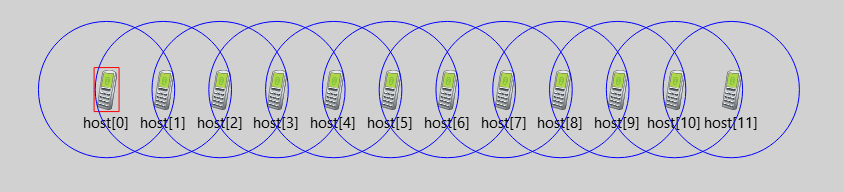
\includegraphics[scale=0.75]{img/singleQueueGUI.png}
        \caption{Validation configuration with 12 hosts placed on a line}
        \label{fig:single_queueGUI}
    \end{center}
    \vspace*{-0.8cm}
\end{figure}

In this configuration, host[0] always broadcasts during the first slot and then the message travels along the queue, with a total of 10 hops. On every hop, the per-slot probability of successful transmission is $p$, which implies an average number of attempts equal to $\frac{1}{p}$. Therefore, the expected coverage time is

\begin{equation}
    E[T] = 1 + 10 \cdot \frac{1}{p}
    \label{eq:singleQueueValidationAvgT}
\end{equation}

Validation was performed with 9 different configurations, one for  each value of $p$ ranging from $0.1$ to $0.9$, with 200 repetitions each.
The following results were obtained:
%TODO replace with plot? Better than table?

\begin{center}
\begin{tabular}{ | m{1cm} | m{5cm}| m{5cm} | }
\hline
$p$& Expected value & Experimental value (mean, interval for 95\% confidence)\\
\hline
$0.1$&$101.0$&$\textbf{99.68}, 95.55, 103.81$\\
\hline
$0.2$&$51.0$&$\textbf{49.9}, 47.93, 51.86$\\
\hline
$0.3$&$34.33$&$\textbf{34.17}, 32.88, 35.46$\\
\hline
$0.4$&$26.0$&$\textbf{25.79}, 24.93, 26.65$\\
\hline
$0.5$&$21.0$&$\textbf{20.84}, 20.24, 21.44$\\
\hline
$0.6$&$17.67$&$\textbf{17.42}, 17.0, 17.84$\\
\hline
$0.7$&$15.29$&$\textbf{15.2}, 14.87, 15.52$\\
\hline
$0.8$&$13.5$&$\textbf{13.48}, 13.25, 13.72$\\
\hline
$0.9$&$12.11$&$\textbf{12.14}, 11.97, 12.3$\\
\hline
\end{tabular}
\end{center}

As can be seen in the table above, %add label to table and reference it?
the experimental results are consistent with the theoretical expected value, with a 95\% confidence level. %rephrase?
\subsection{Star 5-to-1 validation}


\begin{wrapfigure}{r}{0.45\textwidth}
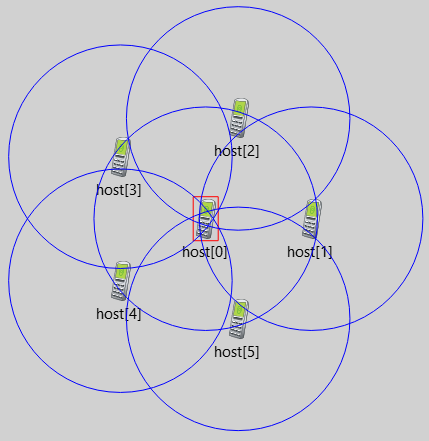
\includegraphics[width=1\linewidth]{img/omnetStar5to1.png} 
\caption{Validation configuration with 5 hosts placed on a star and a target in the middle}
\label{fig:star5to1GUI}
\end{wrapfigure}

In this configuration, host[0] is the target to be reached by the broadcast while all the others already have the message and try to broadcast at every slot with probability $p$.

This system can be modelled by a discrete-time Markov chain, as explained in \ref{ssec:star2}.
The probability of the system to be in the $i$-th state during the $j$-th slot is given by taking the $j$-th power of the stochastic matrix and taking the $i$-th element of the first row.

Validation was performed with 4 different configurations, one for each value of $p$ ranging from $0.2$ to $0.8$ with steps of $0.2$, with 1000 repetitions each.\\
For each configuration, data about the state of the system was recorded and statistics were computed, yielding experimental probabilities. These probabilities were then compared with theoretical predictions, obtained by taking powers of the appropriate stochastic matrix.\\
All the experimental results proved to be consistent with theoretical computations.

\begin{figure}[H]
    \begin{center}
        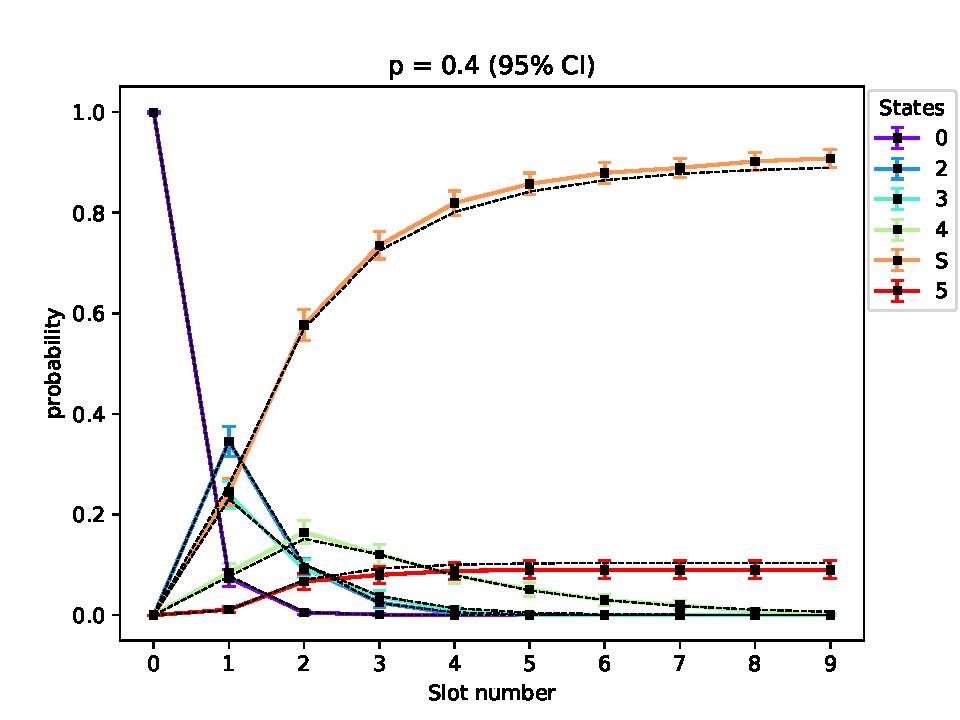
\includegraphics[scale=0.73]{img/star5to1p=0.4validation.pdf}
        \caption{Validation data for p = 0.4}
        \label{fig:5to1validPlot1}
    \end{center}
    \vspace*{-0.8cm}
\end{figure}

%TODO boh c'è spazio, ne ho messo due ma volendo se ne può lasciare solo una
%TODO there's room for two images, we can keep just one if we want

\begin{figure}[H]
    \begin{center}
        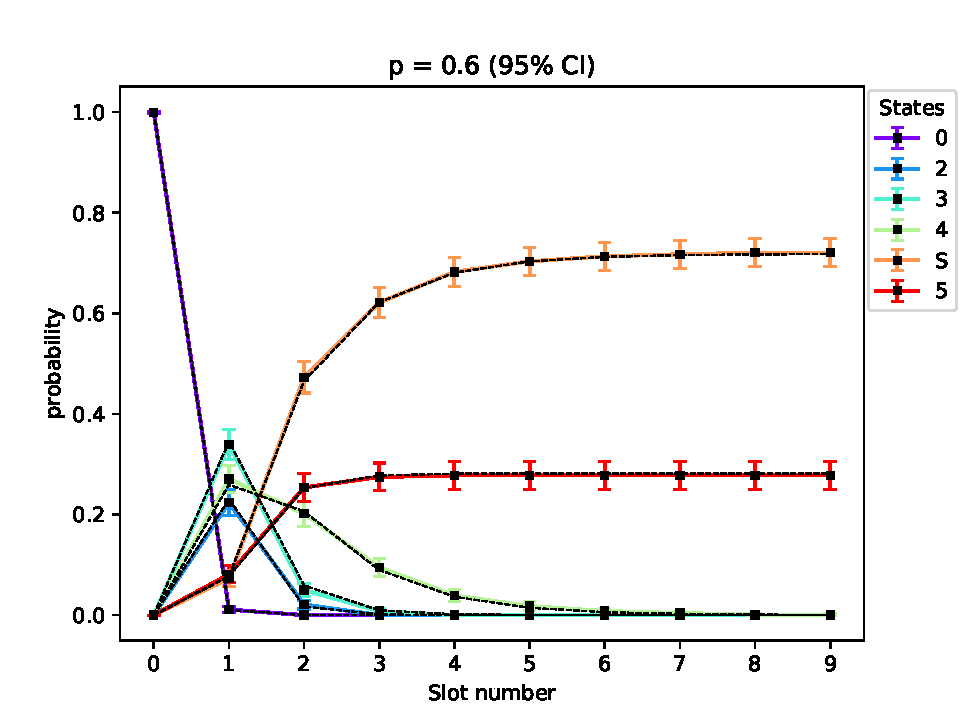
\includegraphics[scale=0.73]{img/star5to1p=0.6validation.pdf}
        \caption{Validation data for p = 0.6}
        \label{fig:5to1validPlot2}
    \end{center}
    \vspace*{-0.8cm}
\end{figure}

Figures \ref{fig:5to1validPlot1} and \ref{fig:5to1validPlot2} show graphs of the experimental data (coloured solid lines) along with predictions (black dashed lines).
%TODO remove empty blank page betwee chapter 4 and 5
%-------------------------------------------------------------------------------
% File: simulation.tex
%       Epidemic Broadcast project documentation.
%
% Author: Marco Pinna, Rambod Rahmani, Yuri Mazzuoli
%         Created on 05/12/2020
%-------------------------------------------------------------------------------
\chapter{Simulation}\label{ch:simulation}
As previously described, the scenario considered was the following:
\begin{itemize}
    \item a $100$m x $100$m floorplan, with the transmission
    radius ranging from $1$ m to $19$ m, with a step of $1$ m, and a Bernoullian RV
    with success probability $p$ ranging from $0.1$ to $0.9$ with steps of $0.1$;
\end{itemize}
\section*{Methodological Note}\label{Methodological}
In order to analyse all the possible combinations for $p$ and $R$, it is necessary to explore the space
generated by the cartesian product of the possible values for each parameter. Every combination 
identifies a scenario, performance indexes need to be computed; in the model
every index is a random variable for which the mean value is sought, with appropriate confidence interval
and confidence level (at least 95\%). 
There were not enough details or prior knowledge on the topic to identify the probability distribution of those variables or even to know if they were symmetric.\\
Nevertheless, some \textit{a priori} considerations could be made about their boundedness and therefore variance: all the indexes are clearly bounded from below, being non-negative. In addition:
\begin{itemize}
    \item \textbf{broadcast time} is bounded from below as the broadcast cannot take less than one slot. Moreover, the worst case scenario is given by a single queue configuration with 100 hosts (see \ref{ssec:singlequeue}); the probability distribution for the broadcast time in this type of scenario is the same geometric distribution as the one for a single transmission, scaled up by a factor equal to the number of hops required. This distribution bounds the broadcast time from above and guarantees a finite variance for it.
    \item the \textbf{percentage of covered users} is bounded from above by 1 (100\%).
    \item the \textbf{number of collisions}, in the case of a floorplan with 100 hosts, is bounded from above by the value 2305. The formula for the upper bound can be found in Appendix B, together with its derivation.
\end{itemize} 
This knowledge allowed for the computation of confidence intervals by means of algorithms that do not require to know the distribution of the
samples but only the finiteness of the variance.
\hfill \break
For each of the scenarios, the floorplan coverage, the
broadcast duration and the number of collisions are measured and plotted in graphs in order to 
better understand and interpret the behaviour of the system.\\
In order to achieve statistically significant results with a minimum accuracy of
$95$\%, each scenario configuration -- with the same parameters -- was run 200 times; then, mean and median values of the performance
indexes were computed, along with their confidence intervals. \\
The analysis of the results showed that mean and median values tend to converge for all the KPIs.
\section{Coverage}\label{ssec:coverage}
Figure \ref{fig:coveragePR} shows the floorplan coverage achieved as a
function of the success probability $p$, for different values of
the transmission radius $R$. \\
As can be observed, the coverage is maximum
for lower values of $p$; this is due to the fact that a low transmission
probability minimizes the number of collisions, increasing the number of correct
transmissions. For values of $R < 8$ we observe an almost linear behaviour:
collisions are almost absent with such a small transmission radius, since the order of the connected component of the graph is quite low; therefore,
variations of the value of $p$ do not play a fundamental role as far as total coverage is
concerned. For $R \geq 8$ the graph starts getting more and more connected and the achievable coverage
decreases with the increase of $p$, but quite slowly and also it does not
degenerate to $0$; instead it reaches a value between $10$\% and $40$\%.
\begin{figure}[H]
    \begin{center}
        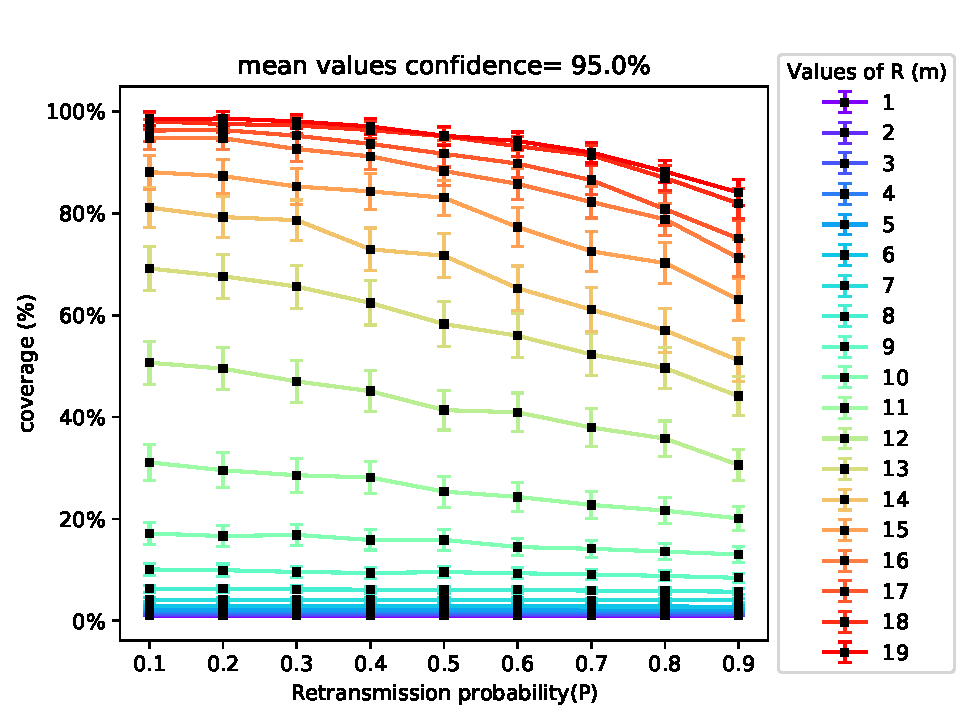
\includegraphics[scale=.62,trim={0 0 0 0.8cm},clip]{img/big_coverage_p_mean_95.0.pdf}
    \end{center}
    \vspace*{-0.5cm}
    \caption{Floorplan coverage as a function of $p$ for different values of $R$}
    \label{fig:coveragePR}
\end{figure}
\noindent
For values of $R$ between $11$ and $15$, the number of collisions has a strong
effect on the coverage percentage; this effect tends to decrease for larger
values of $R$; we know as a matter of fact that for $R \to L\sqrt{2}$ the
coverage tends to $100$\%, independently of any other parameter.\\
\\
Figure \ref{fig:coverageRP} shows the floorplan coverage achieved as a
function of the transmission radius $R$, for different values of the success probability $p$. As expected, accordingly with the previous plot, the
final coverage of the flooplan is deeply influenced by the transmission range $R$.
\begin{figure}[H]
    \begin{center}
        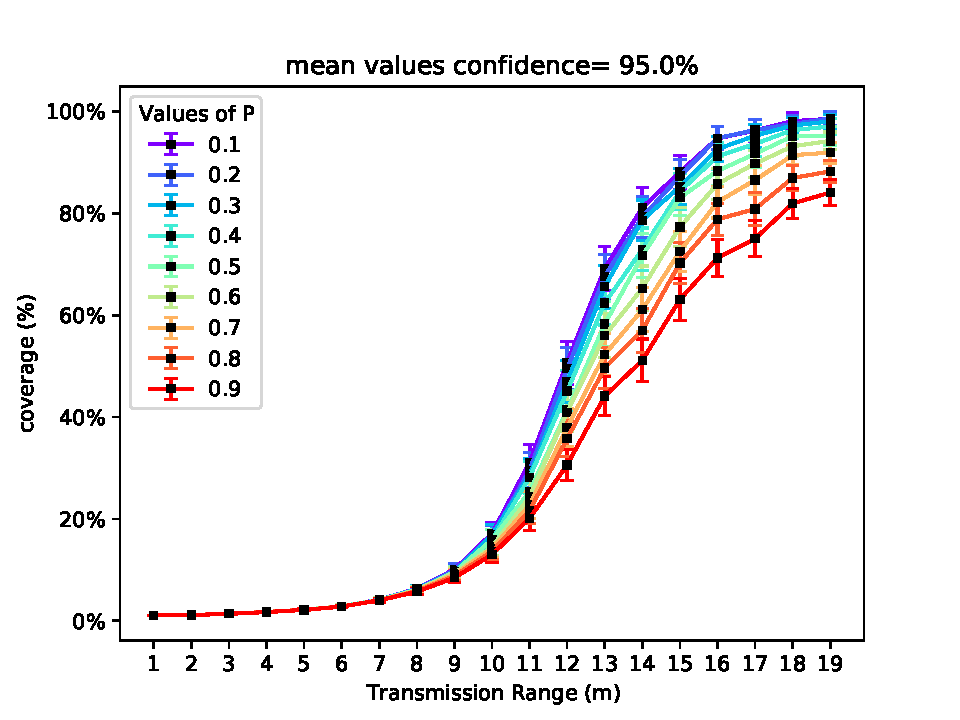
\includegraphics[scale=.75,trim={0 0 0 0.8cm},clip]{img/big_coverage_r_mean_95.0.pdf}
    \end{center}
    \vspace*{-0.5cm}
    \caption{Floorplan coverage as a function of $R$ for different values of $p$}
    \label{fig:coverageRP}
\end{figure}
\noindent

In this second plot we can observe that the coverage increases rapidly
with the transmission range, up to about $R=13$ m. When the transmission range becomes large
($> 16$m) there are diminishing returns, as can be seen by the decreasing steepness of the curves, and the coverage tends to a value of 80-100\%, depending on the value of $p$. The coverage function would appear to be a sigmoid, at least for low values of $R$.\\
A more in-depth analysis is carried out in \ref{ssec:coverageReachSafenodes}.
%increasing and can be manipulated to remain between $0$ and $1$ (like the
%parameter we want to fit). A good fit for this curve is given by:
%\begin{equation*}
%    C = \frac{1+\tanh(aR+b)}{2}
%\end{equation*}
%where $C$ is the floorplan coverage, $R$ the transmission radius, and $a$ and
%$b$ depend on $p$ as shown in the following table:
%\begin{center}
%\begin{tabular}{ | m{1cm} | m{4cm}| m{4cm} | }
%\hline
%$p$&$a$&$b$\\
%\hline
%$0.1$&$0.3628314535334378$&$4.356732935967713$\\
%\hline
%$0.2$&$0.3572920723369711$&$4.3206795324164835$\\
%\hline
%$0.3$&$0.34371134773480694$&$4.193385575628803$\\
%\hline
%$0.4$&$0.3217942874156316$&$3.9814759531755515$\\
%\hline
%$0.5$&$0.3091448275788839$&$3.88645016495332$\\
%\hline
%$0.6$&$0.2809863550485405$&$3.6000814495973996$\\
%\hline
%$0.7$&$0.25932462296148107$&$3.3996924196436975$\\
%\hline
%$0.8$&$0.23603288616377227$&$3.1648817545125527$\\
%\hline
%$0.9$&$0.20917405109220505$&$2.929033169711656$\\
%\hline
%\end{tabular}
%\end{center}
\newpage
\section{Collisions}
Figure \ref{fig:collisionsPR} shows the median number of collisions as function of $p$, for different values of $R$.\\
The values seem to have a linear behaviour for low values of $p$ and then start stabilizing as $p$ approaches one.
\begin{figure}[H]
    \begin{center}
        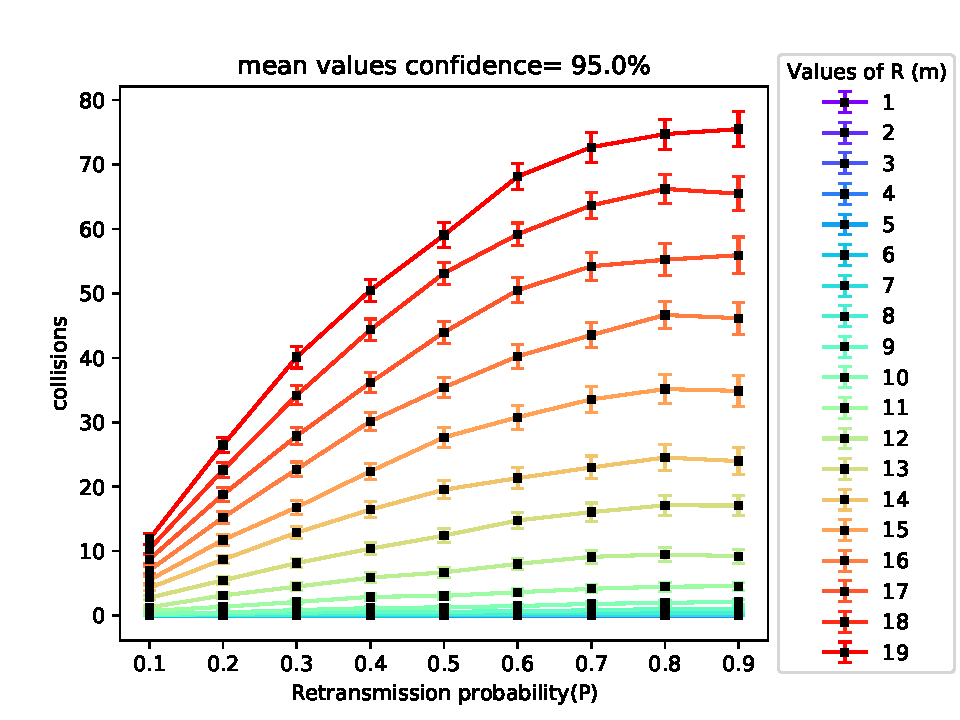
\includegraphics[scale=.7,trim={0 0 0 0.8cm},clip]{img/big_collisions_p_mean_95.0.pdf}
    \end{center}
    \vspace*{-0.5cm}
    \caption{Median value of the number of collisions as function of $R$ for different values of p}
    \label{fig:collisionsPR}
\end{figure}

The dual plot shown in fig. \ref{fig:collisionsRP} provides further insight: low values for $R$ cause no collisions at all, as can also be seen in \ref{fig:collisionsPR} where the lines for $R \leq 8$ all lie on the horizontal axis, regardless of the value of $p$.\\
For bigger values of the radius, the number of collisions grows in a seemingly linear fashion dependent on the value of $R$, with a slope increasing on the increase of $p$.\\
The lines tend to coincide for higher values of $p$, as it also shows the flatness of the curves in the rightmost part of \ref{fig:collisionsPR}.\\
It would incorrect to assert a general positive correlation between the radius and the total number of collisions: as a matter of fact, the number of collisions has to tend to 0 for $R \to \sqrt{2}L$. This is because the more hosts receive the message from host 0, the more of them will be transmitting during the second slot and the less of them will be listening and able to detect a collision.
\begin{figure}[H]
    \begin{center}
        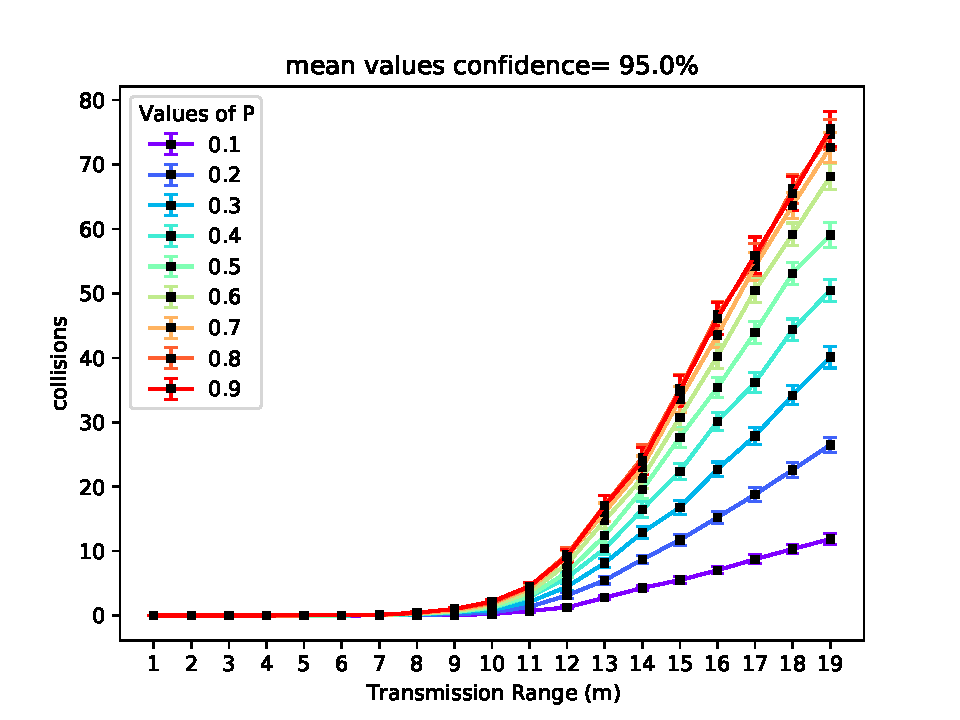
\includegraphics[scale=.65,trim={0 0 0 0.8cm},clip]{img/big_collisions_r_mean_95.0.pdf}
    \end{center}
    \vspace*{-0.5cm}
    \caption{Median value of the number of collisions as function of $R$ for different values of $p$}
    \label{fig:collisionsRP}
\end{figure}
\section{Duration}\label{sec:duration}
The following figure shows the plot of the duration of the simulation (in
slots) as a function of $p$, for different values of $R$.
\begin{figure}[H]
    \begin{center}
        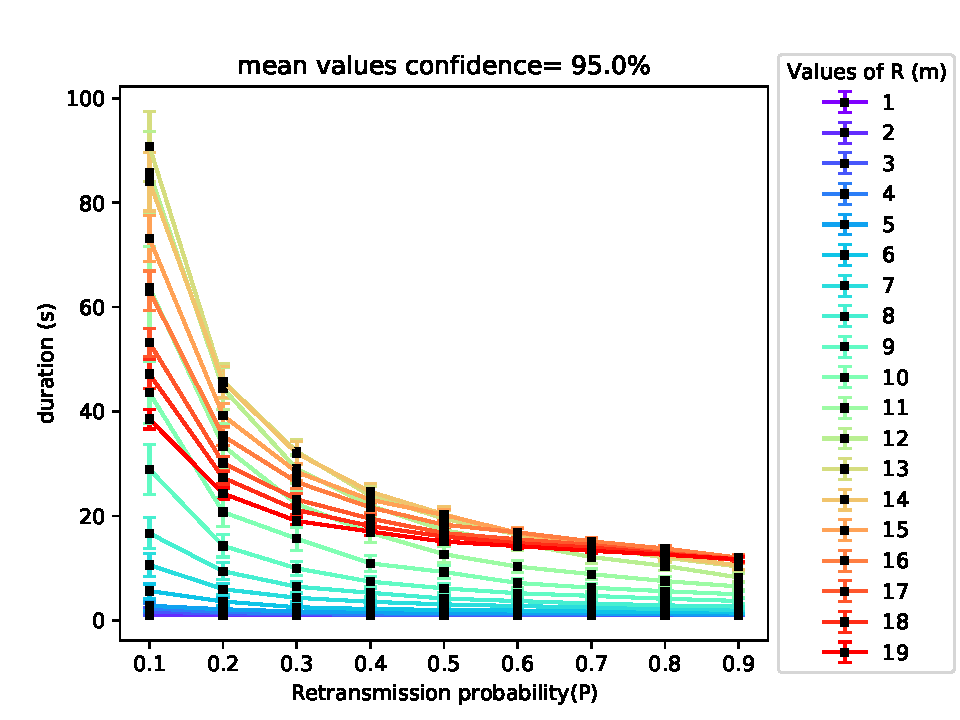
\includegraphics[scale=.67,trim={0 0 0 0.8cm},clip]{img/big_duration (s)_p_mean_95.0.pdf}
    \end{center}
    \vspace*{-0.5cm}
    \caption{Simulation duration as a function of $p$ for different values of $R$}
    \label{fig:durationPR}
\end{figure}
\noindent
The duration of the broadcast increases for lower values of $p$; this behaviour can be
explained as a consequence of two main factors:
\begin{itemize}
    \item the probability of retransmission is low, hence nodes will spend more
    time slots waiting, without actually transmitting;
    \item with a smaller number of collisions, fewer paths are ``cut off" while the message is travelling along them; this causes the message to stay around for a longer time.
\end{itemize}
\begin{figure}[H]
    \begin{center}
        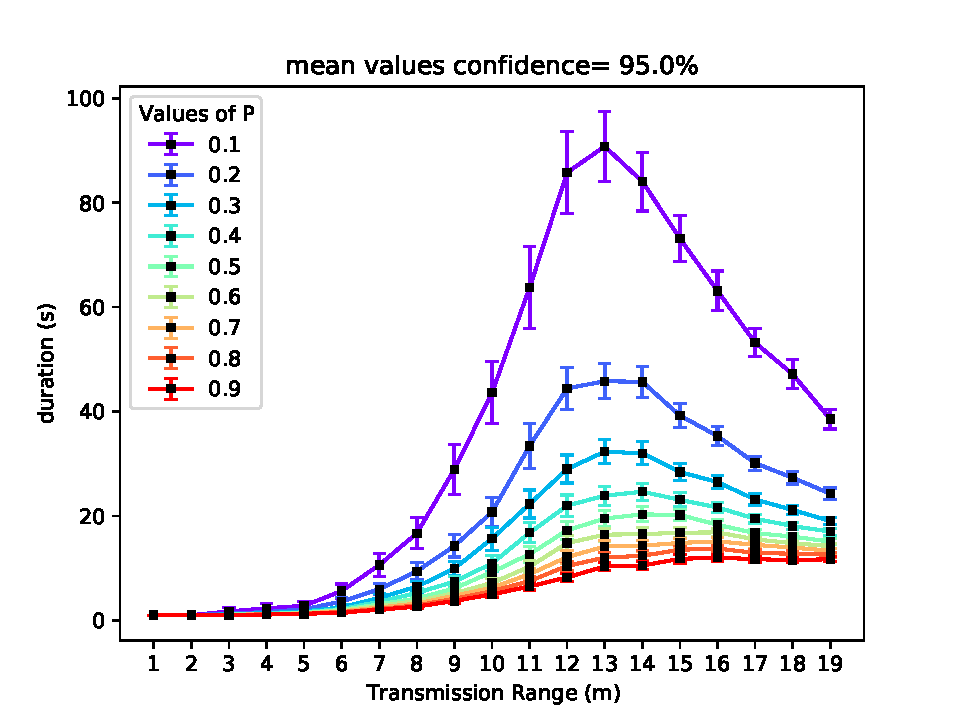
\includegraphics[scale=.7,trim={0 0 0 0.8cm},clip]{img/big_duration (s)_r_mean_95.0.pdf}
    \end{center}
    \vspace*{-0.5cm}
    \caption{Simulation duration as a function of $R$ for different values of $p$}
    \label{fig:durationRP}
\end{figure}
\noindent

The plot in fig. \ref{fig:durationRP} is the dual of the one shown in \ref{fig:durationPR} and shows the duration of the simulation (in slots) as a
function of $R$, for different values of $p$.\\
The duration of the simulation tends to increase with the transmission range,
reaching a peak around $13$ m; the maximum value depends on the probability of
retransmission ($p$) and the distance between the peaks would suggest this dependency to be an inverse proportionality; this would also be consistent with the trend exhibited by the curves in fig. \ref{fig:durationPR}, where the topmost ones resemble hyperbolas.\\
The bottom ones are much flatter, since very low values of $R$ often do not even allow the starting node to be connected to any others.
This supposedly inverse proportionality with respect to $p$ is an interesting result and can be explained by observing that the same inverse proportionality is found in formula \ref{eq:singleQueueMeanT}.\\
Further observation about this and relationship with some graph properties are discussed in \ref{ssec:durationVsEccentricity}.\\
\newpage
Not all the curves in \ref{fig:durationPR} exhibit a hyperbolic trend: very low values of $R$ cause them to have a degenerate trend, while for high values of $R$ the deviation from the hyperbola is likely to be due to the increasing influence of the collisions.
%
%We tried to interpolate the curves shown in Figure \ref{fig:durationPR}
%with an hyperbolic function, because it fits well the parameters we want to
%model; first of all, the hyperbole tends to infinity as $p$ tends to $0$, and
%this is coherent with the reality, because if the probability of retransmission
%becomes low, then the duration keeps increasing. If instead $p$ gets close to
%$1$, the duration time tends to its minimum. We fit those shapes using:
%\begin{equation*}  
%    D = \frac{a}{P}+b 
%\end{equation*}
%where $D$ is the duration of the simulation, $p$ the probability of
%retransmission, and $a$ and $b$ depend on $R$ as specified in the following
%table:
%TODO too many digits. Better to reformat as the wall of text is not exactly pretty
%\begin{center}
%\begin{tabular}{ | m{1cm} | m{5cm}| m{5cm} | }
%\hline
%$R$&$a$&$b$\\
%\hline
%$1$&$2.4046845625846913$ e-09&$0.999999999244136$\\
%\hline
%$2$&$2.4046845625846913$ e-09&$0.999999999244136$\\
%\hline
%$3$&$0.7313966348173997$&$0.9495446821974095$\\
%\hline
%$4$&$1.3471717522270503$&$0.9454326532617134$\\
%\hline
%$5$&$1.7744177255115228$&$1.08724762049118$\\
%\hline
%$6$&$4.652279267805434$&$1.0487610714204172$\\
%\hline
%$7$&$9.586489452244717$&$1.088347295851843$\\
%\hline
%$8$&$15.841670397411658$&$1.0643797063994824$\\
%\hline
%$9$&$28.264640360031194$&$0.49558107430696624$\\
%\hline
%$10$&$43.141734847778814$&$0.22815570364285975$\\
%\hline
%$11$&$64.55944043148898$&$-0.07517936077209139$\\
%\hline
%$12$&$86.56257725232254$&$-0.09919809415424388$\\
%\hline
%$13$&$89.72686483087844$&$1.2578386401845827$\\
%\hline
%$14$&$82.15919574473708$&$3.0965825999956778$\\
%\hline
%$15$&$67.95268283187643$&$5.415446394742158$\\
%\hline
%$16$&$56.442159145137495$&$6.991880399220213$\\
%\hline
%$17$&$45.71412729773696$&$7.548465010848107$\\
%\hline
%$18$&$39.164500694866284$&$7.991652317096266$\\
%\hline
%$19$&$29.71836400235831$&$9.075854630828385$\\
%\hline
%\end{tabular}
%\end{center}
%as a matter of fact, if the transmission range is
%too short nodes can not communicate: they are not in reach by each others.\\
%\\

\section{Comparison between KPIs and graph properties}

Some of the results shown in the previous section can be better understood when compared with some properties of the graphs associated with the configurations of the hosts.\\
In particular, three properties of the graphs have been studied:

\begin{itemize}
	\item the \texttt{reach}, defined as the number of nodes that can be reached from host (vertex) 0. More formally, let $H$ be the connected component containing host 0 of the initial graph $G$, i.e. the induced subgraph in which any vertex is connected to vertex 0. The \texttt{reach} is the \textit{order} of $H$.
	\item the \texttt{eccentricity}, already defined in \ref{sec:graphModelForWirelessSystems}
	\item the number of \texttt{safe nodes}, which has been defined for simulations with $p=1$ as the number of nodes that correctly receive the message. Systems with $p=1$ are completely deterministic and therefore the number of \textit{safe nodes} only depends on the topology of the network.
\end{itemize}

\subsection{Coverage, reach and safe nodes}\label{ssec:coverageReachSafenodes}

In \ref{ssec:coverage} results about the coverage were shown and it was hypothesized that this index, as function of $R$, might have a sigmoidal trend.\\
Let us consider the limit case where $p \to 0$.\\
As $p$ approaches 0, during each slot it becomes less and less likely for an active node to transmit the message. On the other hand, smaller values of $p$ lower the probability of collisions even more.\\
For values of $p$ really close to 0, it is easy to imagine that there will be basically no collisions; at the same time, every node belonging to the connected component of node 0 will sooner or later receive the message with a probability of 1.\\
\begin{figure}[H]
	\begin{minipage}{.5\textwidth}
        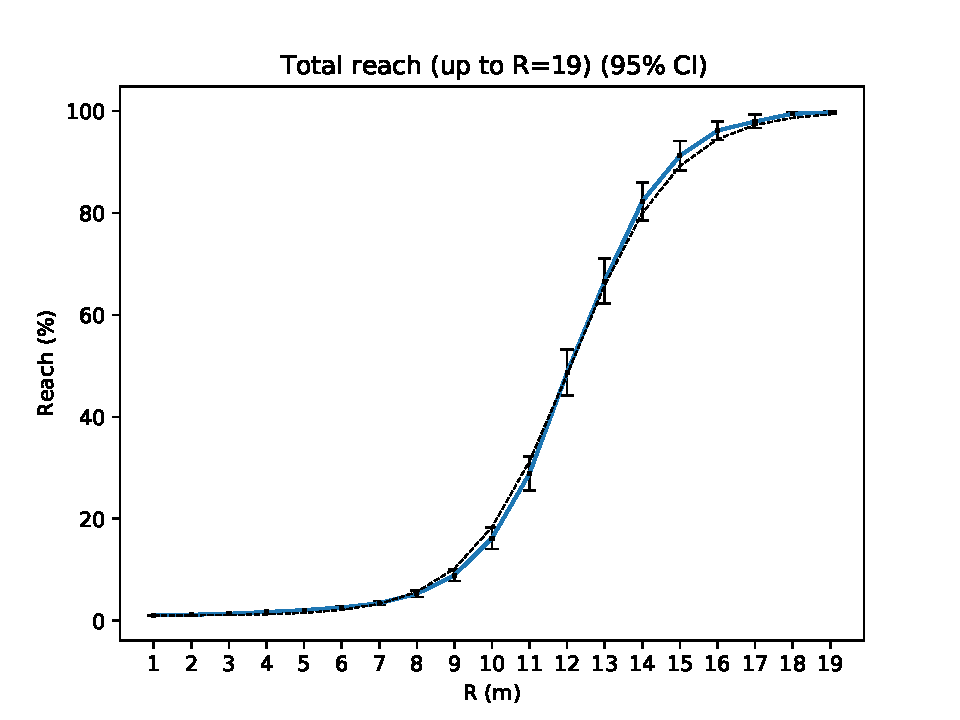
\includegraphics[scale=.5]{img/graphAnalysisTotal_reachR19.pdf}
        \begin{center}
            a)
        \end{center}
	\end{minipage}
	\begin{minipage}{.5\textwidth} 
		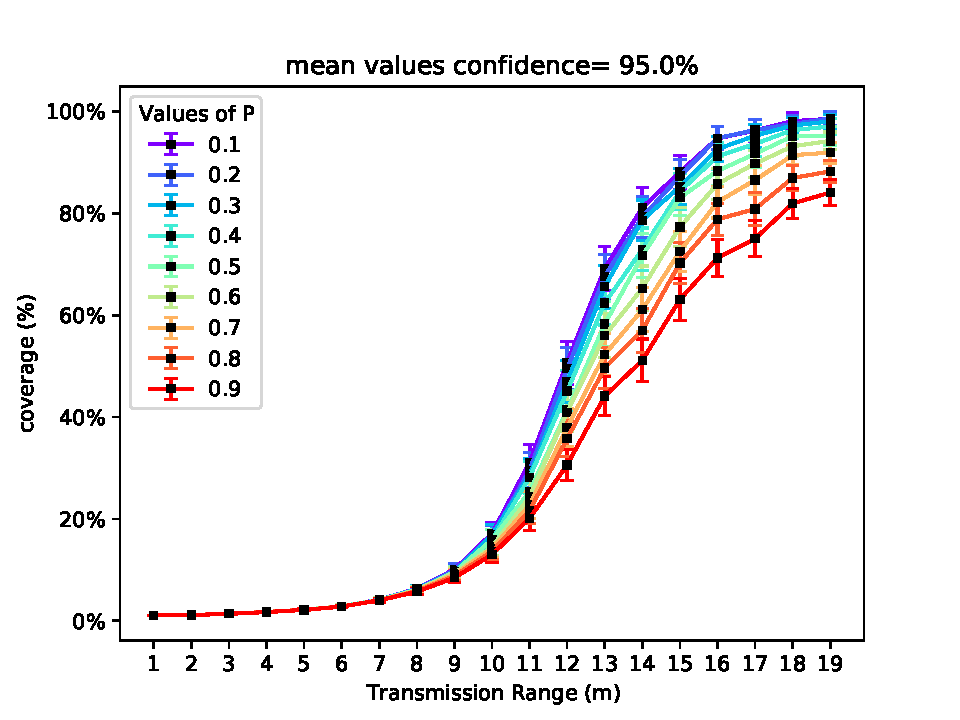
\includegraphics[scale=.5]{img/big_coverage_r_mean_95.0.pdf}
		\begin{center}
            b)
        \end{center}
	\end{minipage}
	\caption{}
    \label{fig:reachR30}
\end{figure}
\hfill \break
\hfill \break
Figure \ref{fig:reachR30} a) shows the average reach from node 0, as function of $R$, in a graph with 100 nodes and figure \ref{fig:reachR30} b) the experimental data for the coverage, for convenience of comparison. The plot in \ref{fig:reachR30} a)  plateaus at a value of 100 for values of $R \geq24$ metres. \\
Various sigmoid functions have been tested to fit the experimental values for the \textit{reach}, and the most appropriate one was found to be
\hfill \break
\begin{equation}\label{eq:reachSigmoidParametric}
	S(R) = \frac{1}{N} + \frac{N-1}{N}\cdot\frac{1+tanh(b(R-a))}{2}
\end{equation}
\hfill \break
where $N$ is the number of nodes in the graph, $a$ controls to the abscissa of the inflection point and $b$ controls how steep the increase is.\\
The correct value for $a$ can be found examining the data in fig. \ref{fig:reachR30} and observing that they show an inflection point for $R=12$ m. With regard to parameter $b$, trial and error showed that its value lies between $0.36$ and $0.37$. In fact, a value equal to $e^{-1} \approx 0.36788$ fits the data very well.\\
% and it makes sense in the presence of a hyperbolic tangent function ?
A closed form for the \textit{reach}, and therefore for total coverage when $p \to 0$, in a square floorplan with $L=100$ would then be
\hfill \break
\begin{equation}\label{eq:reachSigmoidNoL}
	U_{0}(R) = \frac{1}{100} + \frac{99}{100}\cdot\frac{1+tanh(e^{-1}(R - 12))}{2}
\end{equation}
\hfill \break
This formula, however, models the coverage for a fixed values of \texttt{L} and $N$, as mentioned above.\\
A more complete closed form, that also takes in account the length of the side of the floorplan and the number of hosts, might be the following:
\hfill \break
\begin{equation}\label{eq:reachSigmoidL}
	U_{0}(R, L, N) = \frac{1}{N} + \frac{N-1}{N}\cdot\frac{1+tanh(e^{-1}(10\sqrt{N}\frac{R}{L} - 12))}{2}
\end{equation}
\hfill \break
The presence of the quantity $\frac{R}{L}$ follows from the observation that the overall connectivity of a graph should only depend on the ratio between the transmission radius and the coordinates of the hosts (see section \ref{sec:graphModelForWirelessSystems}).\\
The rationale behind the $\sqrt{N}$ term is that the average number of nodes per unit area goes with the \textbf{square} of $N$, and supposedly also does the average number of nodes per transmission circle.\\
Another way to visualize this is to imagine the entire graph in a $L$x$L$ floorplan, divide the floorplan in four $\frac{L}{2}$x$\frac{L}{2}$ squares and take the graph that lies in one of these squares: on average it will have a fourth of the initial number of nodes but its level of connectivity should presumably be the same as the original graph.\\
The value for $a$, as mentioned above, was found by observing experimental data and it is, almost certainly, not an exact value.\\
Lastly, coverage is also likely to depend on the shape of the floorplan itself, which is not taken in account in the formula. Further research is needed\\
\hfill \break
Let us now consider the limit case where $p \to 1$.\\
The closer $p$ gets to $1$, the more the system approaches a deterministic behaviour where each active host broadcasts the message as soon as it receives it.\\
When $p=1$ the number of node that correctly receive the message during the broadcast can be computed by knowing only the topology of the network.\\
\begin{figure}[H]
    \begin{center}
        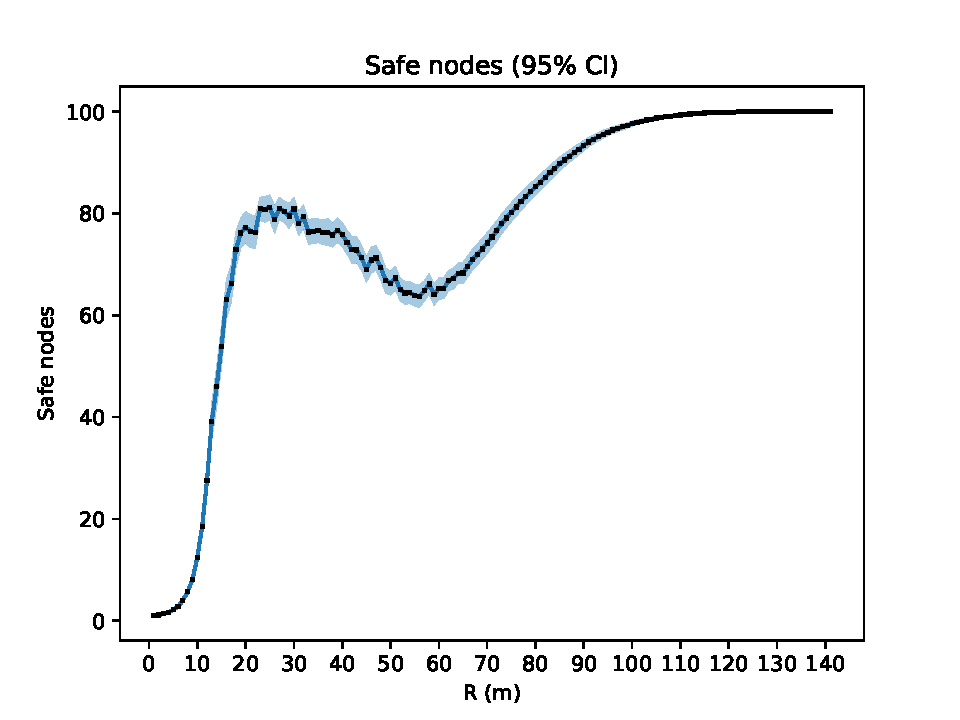
\includegraphics[scale=.6]{img/graphAnalysisSafe_nodes.pdf}
    \end{center}
    \vspace*{-0.5cm}
    \caption{Average number of safe nodes of a graph as function of R}
    \label{fig:safeNodes}
\end{figure}
\hfill \break
Figure \ref{fig:safeNodes} shows the average number of safe nodes during a broadcast starting from node 0, as function of $R$, in a graph with 100 nodes.\\
It is clear that this function does not have a sigmoidal trend, except for low values of $R$, up to about 25 metres, where the number of safe nodes reaches about 80. This is consistent with the trend of the curve for $p=0.9$ in Figure \ref{fig:coverageRP} shown in the previous section.\\
For $R > 25$, increasing the radius yields negative returns: the average number of safe nodes decreases until $R$ reaches about 55 metres. This is likely to be due to the fact that the increase in the number of collision takes over on the increase of reachable nodes. This is consistent with the hypothesis made in Chapter \ref{ch:overview} when analysing the impact of $R$ on the KPIs.\\
For $R > 55$ the number of safe nodes starts increasing again, probably because host 0 starts having more and more neighbours when the broadcast begins (and none of them detects a collision as host 0 is the only one transmitting during the first slot).\\ The quantity asymptotes to the total number of nodes and for $R > \sqrt{2}{\cdot}L$ it is identically equal to it since, wherever the starting node would happen to be placed, it would cover the whole area during its first transmission slot.\\
\hfill \break
These considerations show that the coverage as function of $R$, although it might resemble a sigmoid for different values of $p$ (and could probably be approximated well enough by it for realistic value of the transmission range), is probably more complex than that; for a certain range of values for R, the increase in the number of collision starts having a heavier role in the number of reached hosts.\\
A closed formula for the number of safe nodes when $p=1$ has not been found yet but, assuming it is $C_{1}(R)$, then a reasonable form for the coverage function could be the following:
\begin{equation}\label{eq:coverageClosedForm}
C(R, p) = (1-p)\cdot C_{0}(R) + p\cdot C_{1}(R)
\end{equation}

\subsection{Broadcast time and eccentricity}\label{ssec:durationVsEccentricity}
In \ref{sec:graphModelForWirelessSystems} the eccentricity $\epsilon$ of a graph was introduced, defined as the distance from node 0 to the furthest connected node, let it be $u$.\\
If we imagine the message spreading from host 0 outwards along the various paths of the graph, it is easy to guess that, on average, the path that will take the longest to be covered will be the one that leads to node $u$ and this path will have, by definition, a number of edges equal to the eccentricity.\\

\begin{figure}[H]
    \begin{center}
        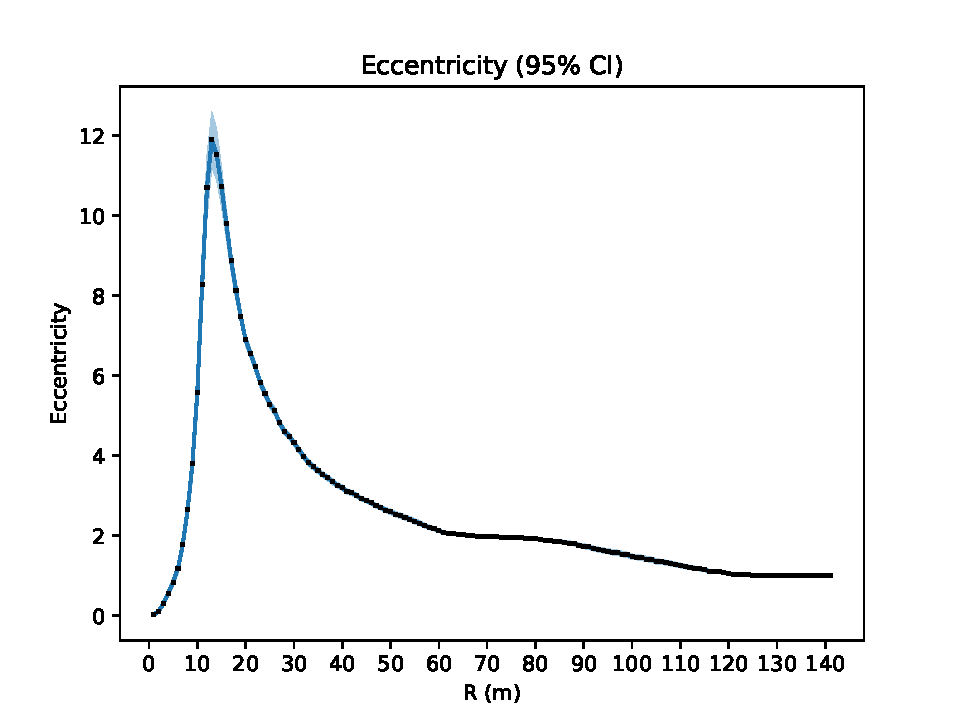
\includegraphics[scale=.6]{img/graphAnalysisEccentricity.pdf}
    \end{center}
    \vspace*{-0.5cm}
    \caption{Average number of safe nodes of a graph as function of R}
    \label{fig:eccentricityFull}
\end{figure}
\hfill \break
Figure \ref{fig:eccentricityFull} shows the average eccentricity of a graph with 100 nodes, as function of R.
The function has a maximum around $R = 13$ m and then starts slowly decaying until it reaches 1 as R gets closer to $\sqrt{2}L$; this makes complete sense since, for high values of R, node 0 is quite likely to be connected to all nodes in the floorplan.\\
The peak at $R=13 m$ has the following physical interpretation: for values of R between 0 m and 13 m, increasing the radius increases the order of the connected component of the graph containing node 0; by further increasing the radius, more edges start to appear in the graph creating shorter paths between nodes that were already connected.\\
Another interesting observation concerns the behaviour of the function around $R = 70$ m: the eccentricity seems to stabilize at a value of 2, with very narrow confidence intervals, for values  of $R$ close to $\frac{1}{2}\sqrt{2}L$.\\
Fig. \ref{fig:eccentricityDuration} shows the previous function up to $R=19$ m one one side, and again the experimental data for the duration, for convenience of comparison.\\
\begin{figure}[H]
	\begin{minipage}{.5\textwidth}
        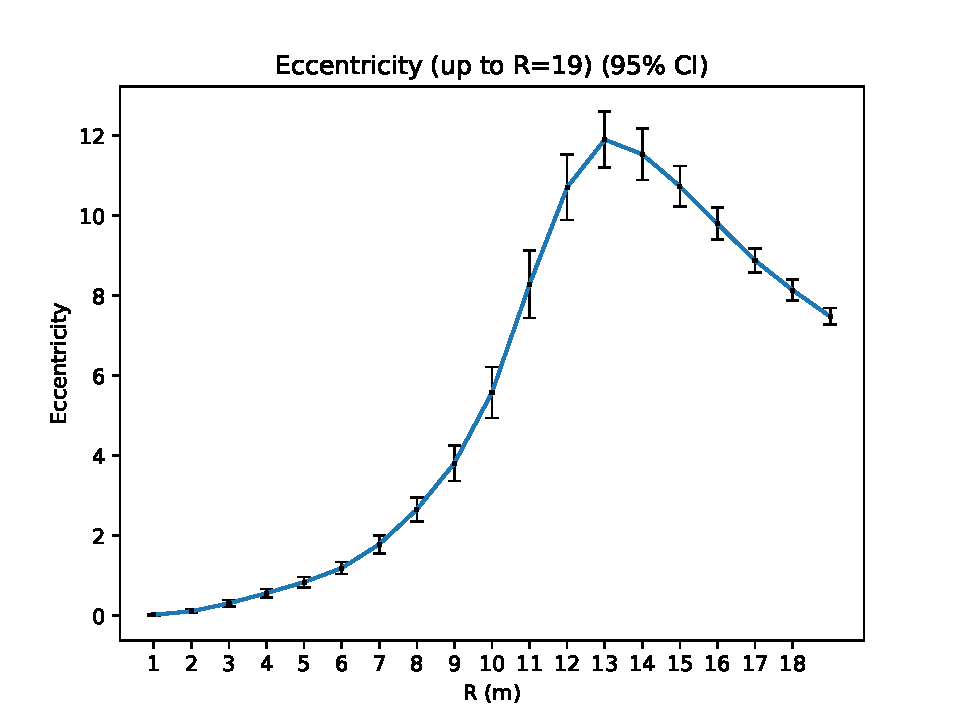
\includegraphics[scale=.5]{img/graphAnalysisEccentricityR19.pdf}
        \begin{center}
            a) Eccentricity as function of R
        \end{center}
	\end{minipage}
	\begin{minipage}{.5\textwidth} 
		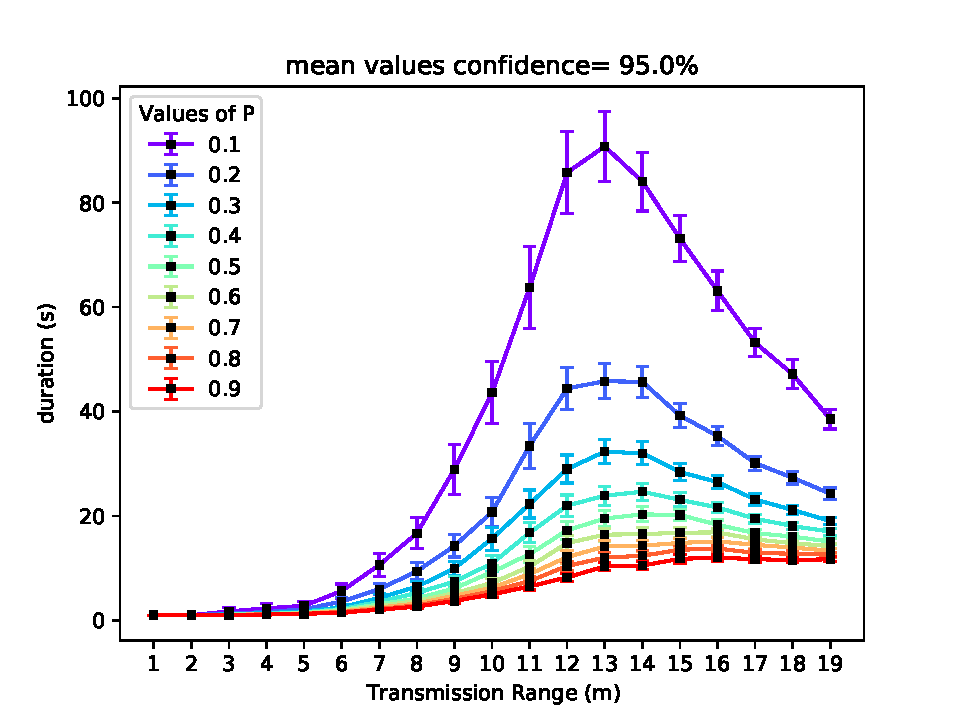
\includegraphics[scale=.5]{img/big_duration (s)_r_mean_95.0.pdf}
		\begin{center}
            b) Broadcast time as function R
        \end{center}
	\end{minipage}
	\caption{}
    \label{fig:eccentricityDuration}
\end{figure}
\hfill \break
The curves on the right clearly resemble the one on the left, minus a scaling factor, especially for lower values of $p$.\\
As the value of $p$ approaches one, the curves tend to flatten and this might be due to the fact that the number of collision increases and more paths are cut off (see \ref{sec:duration}).\\
The spacing between the duration curves might suggest that this scaling factor is the inverse of the corresponding $p$, as mentioned earlier. This would make complete sense because the average time a message takes to travel along a path of $n$ hops is $n \cdot \frac{1}{p}$ (see \ref{ssec:singlequeue}).\\
In fact, while the spacing does indeed suggest an inverse dependency on $p$, the actual values turn out to be about 20\% smaller. The existence of this additional $\sim0.8$ scaling factor could be motivated as follows:\\
the eccentricity of a graph gives information about the longest path from a node to the furthest node $u$, but does not say anything about the number of paths of that length. In the graph there might very well be different paths of length $\epsilon$ that connect node 0 to $u$, either completely disjunct or with some nodes in common and ``forks", ``branch-ins" and ``branch-outs". If these paths happens to be disjunct, node $u$ will receive the message as soon as it arrives from the ``fastest" one. 

\begin{wrapfigure}{r}{0.45\textwidth}

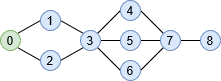
\includegraphics[width=1\linewidth]{img/branchIn.png} 
\caption{Example of graph with multiple shortest path of lenght $\epsilon$}
\label{fig:branchIn}
\end{wrapfigure}

If the paths happen to have nodes in common, as it is the case in fig. \ref{fig:branchIn}, every time there is a ``branch-in" ($[1,2]{\to}3$ or $[4,5,6]{\to}7$ in the figure) there is a possibility that the message will have a speed ``boost" with respect to its average speed along a single queue and also a possibility that its progress will be interrupted by a collision.

\section{Performance optimization}
The ultimate goal of this study is to find the optimal configuration of parameters to ensure the highest coverage in the lowest possible time, since the message should ideally reach all the users as soon as possible.\\
The trivial solution is to make the transmission radius so big that it covers the entire floorplan, thus ensuring total coverage in one single slot.
This is clearly not viable if the floorplan size gets really big.\\
If one wishes to only maximize the coverage, regardless of the amount of time it would take to reach the last user, they should choose the biggest $R$ the devices allow for and a low value of $p$: this configuration corresponds to the top right corner of figure \ref{fig:coverageRP}. The downside of this choice of parameters is that the duration of the broadcast will be very long, as shown in the corresponding curve in fig. \ref{fig:durationRP}.\\
If, instead, one wishes to minimize the duration of the broadcast, possibly at the expense of not having full coverage, they should opt for a higher value of $p$. In this case, the choice of $R$ is not as obvious: provided that $R$ cannot be large enough to cover the whole area, it should be ensured that chosen value does not fall within the range that yields negative returns, as discussed in the second part of \ref{ssec:coverageReachSafenodes} and shown below in fig. \ref{fig:safeNodesShaded}. In practical terms, referring to fig. \ref{fig:safeNodes}, if $R$ can be greater than $\sim76$ metres, it should be as high as possible; if it cannot be greater than $\sim76$ metres, then $R$ should be kept at $\sim25$ metres, since higher values would result in a poorer performance.

\begin{figure}[H]
    \begin{center}
        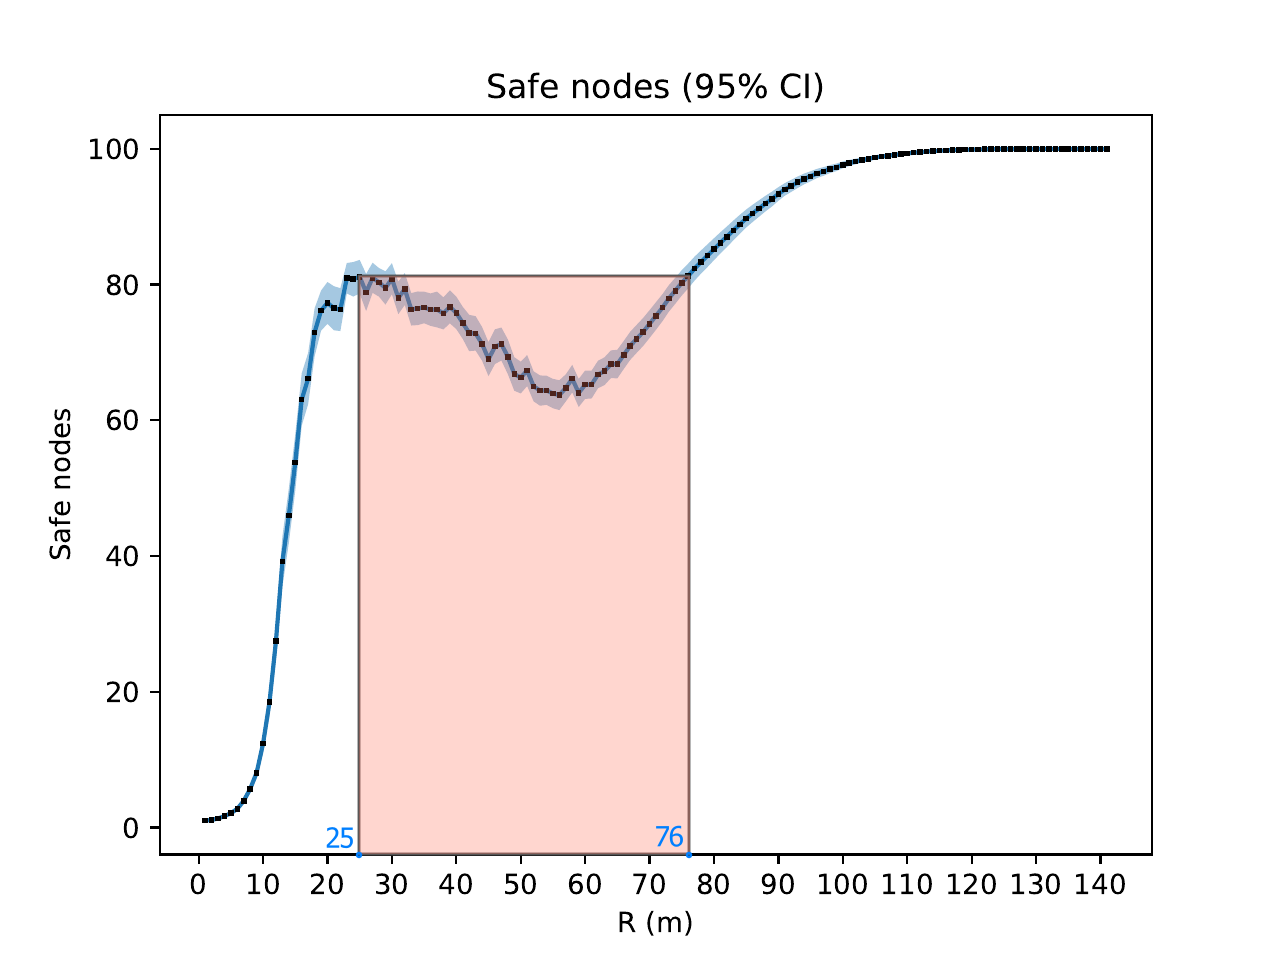
\includegraphics[scale=0.7]{img/graphAnalysisSafe_nodesRed.png}
        \caption{}
        \label{fig:safeNodesShaded}
    \end{center}
    \vspace*{-0.8cm}
\end{figure}
%-------------------------------------------------------------------------------
% File: appendicies.tex
%       Epidemic Broadcast project documentation.
%
% Author: Marco Pinna, Rambod Rahmani, Yuri Mazzuoli
%         Created on 05/12/2020
%-------------------------------------------------------------------------------
\chapter{Appendices}
\section{Appendix A}
\label{app:a}
Given a scenario with $N$ transmitter devices and one target device $T$ in reach
by all of the transmitter devices, let us define the probabilities $P_{1}(j, N)$
as the probability of $j$ devices out of $N$ transmitting at the same time
during the time slot $1$ and $P_{i}(j)$ as the probability of $j$ devices
transmitting at the same time during slot $i$.\\
By specification, the successful reception of the message by device $T$ occurs
when \textbf{one} and only one of the transmitters sends the message during the
time slot. Furthermore, the successful transmission of a device is
``\textit{a Bernoullian RV with success probability \emph{p} on every slot, until
it achieves success}". Therefore, we can model $P_{1}(j, N)$ as follows:
\[
\begin{drcases}
    &P_{1}(0, N) = (1-p)^{N} \\
    &P_{1}(1, N) = N p(1-p)^{N-1}\\
    &P_{1}(2, N) = {N\choose2}p^{2}(1-p)^{N-2}\\
    &P_{1}(3, N) = {N\choose3}p^{3}(1-p)^{N-3}\\
    &...\\
    &P_{1}(N-1, N) = {N\choose N-1}p^{N-1}(1-p)\\
    &P_{1}(N, N) = {N\choose N}p^{N}\\
\end{drcases}
P_{1}(j, N) = {N\choose j} p^{j} (1-p)^{N-j}
\]
As for $P_{i}(j)$ we can model the system as if it was in the first time slot,
with the total number of active devices now being equal to $N - t$, where
$t$ is the number of devices that have transmitted in the $(i - 1)$-th slot.\\

\newpage
\section{Appendix B}
\label{app:b}
An example of stochastic matrix for a system with $N = 5$ and $p = 0.4$:
\begin{equation*}
P = 
\begin{bmatrix}
P_{0,0}	& P_{0,2}	& P_{0,3}  	& P_{0, 4}	& P_{0,S}	& P_{0,5} \\
		& P_{2,2}	& 0  		& P_{2, 4}	& P_{2,S}	& P_{2,5} \\
		& 			& P_{3,3}	& 0			& P_{3,S}	& P_{3,5} \\
		& 			& 			& P_{4,4}	& P_{4,S}	& 0\\
		& 			& 			& 			& 1			& 0\\
0		& 			& 		  	& 			& 			& 1\\
\end{bmatrix}
\label{exampleMatrix}
\end{equation*}
Here with numerical values (rounded to 4 decimal places):

%P = 
%\begin{bmatrix}
%0.0778	& 0.3456	& 0.2304  	& 0.0768	& 0.2592	& 0.0102 \\
%		& 0.216		& 0  		&0.288		& 0.432		& 0.064 \\
%		& 			& 0.36		& 0			& 0.48		& 0.16 \\
%		& 			& 			& 0.6		& 0.4		& 0\\
%		& 			& 			& 			& 1			& 0\\
%0		& 			& 		  	& 			& 			& 1\\
%\end{bmatrix}

\begin{equation*}
P=
\begin{blockarray}{ccccccc}
 & 0 & 2 & 3 & 4 & S & 5 \\
\begin{block}{c[cccccc]}
0	&	0.0778	& 0.3456	& 0.2304  	& 0.0768	& 0.2592	& 0.0102 \\
2	&			& 0.216		& 0  		&0.288		& 0.432		& 0.064 \\
3	&			& 			& 0.36		& 0			& 0.48		& 0.16 \\
4	&			& 			& 			& 0.6		& 0.4		& 0\\
S	&			& 			& 			& 			& 1			& 0\\
5	&	0		& 			& 		  	& 			& 			& 1\\
\end{block}
\end{blockarray}
\label{exampleMatrixValues}
\end{equation*}
\newpage
\section{Appendix C}
\label{app:c}
Given a generic convex shape as floorplan, we can compute its area ($A$); if we
imagine placing a point mass transmitter (\texttt{trx}) in a random point of
such floorplan, it is easy to compute the probability for \texttt{trx} to be
located in a given point \textit{x} as:
%TODO fix, a probability cannot be a density, it should turn out to be an adimensional number. Furthermore, if we consider the coordinates to be real number, the probability is zero in every point.
\begin{equation*}
    P(x) = 1/A
\end{equation*}
Given that the transmission radius in $r$, we can define a circle centered in x, 
as the transmission range of the first \texttt{trx} ($R$). If the \texttt{trx}
in far enough from the border of the floorplan, its whole transmission circle lies
onto the floorplan; in this case, the probability for another (random
positioned) \texttt{trx} to be placed inside within its range is equal to:
\begin{equation*}
    P(x') = \int_{R}^{} P(x)= \frac{2\pi r^2}{A} \ 
\end{equation*}
If the first \texttt{trx} device is placed at a distance less than $r$ from one
or more borders of the floorplan, the probability of randomly placing another
\texttt{trx} device in its range is less than in the previous case; this is
because part of the area of the transmission range will fall out of the
floorplan and, by construction, \texttt{trx} devices can't be placed there. 
Depending on the floorplan' shape, we can identify the partition of the shape
where the transmission range will fall out of the shape itself, and we will do
specific computation for this area.\\
In general, by the middle value theorem for integrals, and the total probability
theorem, the probability for $2$ transmitters (let $x$ and $y$ be their
coordinates) randomly placed to be close enough to be able to communicate is:
\begin{equation*}
    \rho = P(|x-y|<r) = \frac{1}{A} \int_{A}^{} P(x')
\end{equation*}
Since we know that $P(x')$ is not constant for all the area of the shape, this
integral might be difficult to compute, even for a square floorplan; in any case
its value, it's constant for a given floorplan and a given $r$. Taking into
consideration only one \texttt{trx}, we can compute the probability density
function for the number of \texttt{trx} in its transmission range, in function
of the number of \texttt{trx} in the entire floorplan $C(N)$. Every time we put
a \texttt{trx} in the floorplan, the probability that it falls in the
transmission range of the highlighted one is $\rho$. This is true for every
$N > 1$, because of independence.
\begin{equation*}
    C(N)= \left(\frac{1}{p}\right)^{\left( N-1 \right)}
\end{equation*}
This is a Bernoullian distribution, and we can use this result only taking one
\texttt{trx} at time; in other words we cannot use this distribution for all the
\texttt{trx} in a random configured floorplan, because they are not independent. 
The distribution for one \texttt{trx} will be influenced by the position of
others. Anyway, we can apply this distribution to many transmitters, each one
taken from a different floorplan; in this way we can validate the independence
of different random configurations.

\section{Appendix D}
\label{app:d}
Below is a demonstration of the upper bound for the number of collision in a scenario with N hosts.

\hfill \break
The necessary condition for a collision to happen is that at least two hosts transmit during the same slot. Each host placed in the intersection of the transmission circles of the two transmitting hosts detects one collision. \\
Therefore, to maximize the number of collisions, it is necessary in every slot, both to a) maximize the number of hosts that detect the collision and b) minimize the number of transmitting hosts (while still assuring that a collision can happen) so that during the next slot the number of hosts available to detect a collision is the highest.

\hfill \break
Let us suppose to have a floorplan with 100 hosts.\\
\begin{itemize}
	\item
	During slot n. 1, host 0 transmits and, being the only host transmitting, absence of collision is ensured. Let us suppose that the message is received by host 99 and host 98.
	\item
	During slot n. 2, host 99 and host 99 broadcast the message and, out of the 97 active hosts, only host 97 and host 96 receive the message correctly. The remaining 95 detect a collision.
	\item
	During slot n. 3, host 97 and host 96 broadcast the message and, out of the 95 active hosts, only host 95 and host 95 receive the message correctly. The remaining 93 detect a collision.
	\item
	And so on...

\end{itemize}
\hfill \break
Following this line of reasoning, the number of listening hosts decreases by two every slot, and so does the number of collisions.\\
When only 5 hosts are remaining on the floorplan, 2 of which are transmitting and the other 3 are receiving, 2 of the latter 3 receive the message correctly and the last one detects a collision.\\
Finally, the last 2 out of 3 broadcast the message and the last one detects a collision again.
\hfill \break
The total number of collision is therefore $95+93+91...+3+1\textbf{+1} = 2305$.

\hfill \break
It is trivial to prove that if $N \leq 3$, no collisions can happen.
\hfill \break
In general, for a configuration with N hosts, $N \geq 4$, the upper bound for the number of collision is given by the following formula:

\begin{equation}
\label{eq:collisionUpperBound}
	C_{max}(N) = \begin{cases}
	1+(\frac{N}{2}-2)^2 &\text{if N is even}\\
	2+(\frac{N-1}{2} - 2)(\frac{N-1}{2}-1) &\text{if N is odd}
	\end{cases}
\end{equation}

\printbibliography

\end{document}
